% We define graph weight in Section\ref{sec:subgraph_counting_antipattern:interpretation} and introduce non-increasing rules in Section~\ref{sec:subgraph_counting_antipattern:non-increasing}. Using these concepts, Section~\ref{sec:subgraph_counting_antipattern:termination} outlines the methodology and termination criterion.

% \subsection{Generalized ruler-Graphs}
% \label{sec:subgraph_counting_antipattern:interpretation}
% Like using rulers to measure physical objects, we use ruler-graphs (special reference structures) to measure graphs.
% Each ruler-graph in a set $\mathbb{X}$ provides a measure for a graph
% G, and the total weight of G is determined by a weighted linear
% combination of these measures.
% \todo{explain the difference the concept of ruler-graph presented in this paper and the one in the paper of \cite{qiu2025termination_icgt}.}

We use a definition of ruler-graph more general than the one in~\autoref{chap:subgraph_counting}.

\begin{definition}[Ruler-graph]
    A \textbf{ruler-graph} is either $(X)$ or \( (X, f) \) where $X$ is a graph, called \textbf{underlying graph}, and $f$ is a graph monomorphism with $\operatorname{dom}(f) = X$, called the \textbf{forbidden context}.
\end{definition}
For $\mathcal{X} = (X, f:X \rightarrowtail F)$, we will also called $F$ the forbidden context.

% \begin{notation}
%     $\operatorname{MonoNF}((X,F_X), G) = $
% \end{notation}
\begin{definition}[Measurement]
    % \textcolor{red}{
    Let \( \mathcal{X}\) be a ruler-graph and \( G \) a graph. The \textbf{measurement} of \( G \) with respect to \( \mathcal{X}\), denoted \( m_\mathcal{X}(G) \), is defined as 
    \[
        m_\mathcal{X}(G) =
        \begin{cases}
            \card{\{h \in \operatorname{Mono}(X,G) \mid \nexists g.\,f \star g = h \}}, & \text{if } \mathcal{X} = (X, f), \\
            \card{\operatorname{Mono}(X,G)}, & \text{if } \mathcal{X} = (X).
        \end{cases}
    \]
\end{definition}
The novelty over~\autoref{chap:subgraph_counting} is that, for a given ruler-graph, the occurrences of the underlying graph that overlap with its forbidden context are excluded. The definitions of weight function and graph weights do not change.
% \begin{definition}[Weight function]
%     \label{def:weight_function}
%     A \textbf{weight function} for a set of ruler-graphs \( \mathbb{X} \) is a map \( s_{\mathbb{X}} \colon \mathbb{X} \to \mathbb{N} \).
%     %  assigning a weight in $\mathbb{N}$ to each ruler-graph.
% \end{definition}
% \begin{definition}[Graph weight]
%     \label{def:subgraph_counting_antipattern:graph_weight}  
%     Given a set of ruler-graphs \( \mathbb{X} \), 
%     a weight function \( s_{\mathbb{X}} \), and a graph \( G \), the \textbf{weight of graph} \( G \) relative to \( s_{\mathbb{X}} \), written \( w_{s_{\mathbb{X}}}(G) \), is: 
%     \[
%         w_{s_{\mathbb{X}}}(G) = \sum_{\mathcal{X} \in \mathbb{X}} s_{\mathbb{X}}(\mathcal{X}) \cdot m_\mathcal{X}(G)  
%     \]   
% \end{definition}

% \subsection{Non-increasing rules}
% \label{sec:subgraph_counting_antipattern:non-increasing}
% % We use \( S \uplus S' \) to denote the disjoint union of sets \( S \) and \( S' \). Let \( \rho = (L \overset{l}{\leftarrowtail} K \overset{r}{\rightarrowtail} R) \) be a rule.
% \newline
% \noindent
%     \begin{minipage}{0.65\textwidth}
%       The DPO diagram for \( G \Rightarrow_\rho H \) with injective match \( m \) can be seen, up to graph renaming, as a diagram in the category of sets where all morphisms are inclusions. The diagram is shown on the right.
%     \end{minipage}
%     \hfill
%     \begin{minipage}{0.34\textwidth}
%           \hfill
%           \resizebox{0.9\textwidth}{!}{
%             \begin{tikzpicture}
%               \coordinate (k) at (0, 0);
%               \draw[fill=white] ($(k)+(0,0)$) rectangle ($(k)+(0.5,0.5)$);
%               \node () at ($(k)+(0.25,0.25)$) {\( K \)};
          
%               \coordinate (c) at (0, -2);
%               \draw[fill=blue!20]
%               ($(c)+(0,-0.5)$)
%               -- ($(c)+(0,0.5)$) 
%               -- ($(c)+(1,0.5)$) 
%               arc[start angle=0, end angle=-90, radius=1]
%               -- cycle;
%               \node () at ($(c)+(0.7,0.2)$) {\( C' \)};
%               \draw[fill=white] ($(c)+(0,0)$) rectangle ($(c)+(0.5,0.5)$);
%               \node () at ($(c)+(0.25,0.25)$) {\( K \)};
          
%               \coordinate (l) at (-3, 0);
%               \draw[fill=orange!20] ($(l)+(-0.5,0)$) rectangle ($(l)+(0.5,1)$);
%               \node () at ($(l)+(-0.2,0.2)$) {\( L' \)};
%               \draw[fill=white] ($(l)+(0,0)$) rectangle ($(l)+(0.5,0.5)$);
%               \node () at ($(l)+(0.25,0.25)$) {\( K \)};
          
%               \coordinate (g) at (-3, -2);
%               \draw[fill=blue!20]
%               ($(g)+(0,-0.5)$)
%               -- ($(g)+(0,0.5)$)
%               -- ($(g)+(1,0.5)$) 
%               arc[start angle=0, end angle=-90, radius=1]
%               -- cycle;
%               \draw[fill=orange!20] ($(g)+(-0.5,0)$) rectangle ($(g)+(0.5,1)$);
%               \node () at ($(g)+(0.7,0.2)$) {\( C' \)};
%               \node () at ($(g)+(-0.2,0.2)$) {\( L' \)};
%               \draw[fill=white] ($(g)+(0,0)$) rectangle ($(g)+(0.5,0.5)$);
%               \node () at ($(g)+(0.25,0.25)$) {\( K \)};
          
%               \coordinate (r) at (3,0);
%               \draw[fill=red!20] ($(r)+(-0.5,0)$)
%                 -- ($(r)+(-0.5,0.5)$)
%                 -- ($(r)+(0,1)$)
%                 --  ($(r)+(0.5,1)$)
%                 -- ($(r)+(0.5,0)$)
%                 -- cycle;
%               \node () at ($(r)+(-0.2,0.2)$) {\( R' \)};
%               \draw[fill=white] ($(r)+(0,0)$) rectangle ($(r)+(0.5,0.5)$);
%               \node () at ($(r)+(0.25,0.25)$) {\( K \)};
          
%               \coordinate (h) at (3, -2);
%               \draw[fill=blue!20]
%               ($(h)+(0,-0.5)$)
%               -- ($(h)+(0,0.5)$)
%               -- ($(h)+(1,0.5)$) 
%               arc[start angle=0, end angle=-90, radius=1]
%               -- cycle;
%               \draw[fill=red!20] ($(h)+(-0.5,0)$)
%               -- ($(h)+(-0.5,0.5)$)
%               -- ($(h)+(0,1)$)
%               --  ($(h)+(0.5,1)$)
%               -- ($(h)+(0.5,0)$)
%               -- cycle;
%              \node () at ($(h)+(0.7,0.2)$) {\( C' \)};
%              \draw[fill=white] ($(h)+(0,0)$) rectangle ($(h)+(0.5,0.5)$);
%              \node () at ($(h)+(0.25,0.25)$) {\( K \)};
%              \node () at ($(h)+(-0.2,0.2)$) {\( R' \)};
          
%               \node (kl) at ($(k)!0.5!(l)+(0.1,0.2)$) {\( \overset{l}{\leftarrowtail} \)}; 
%               \node (kr) at ($(k)!0.5!(r)+(0.1,0.2)$) {\( \overset{r}{\rightarrowtail} \)};  
%               \node (cg) at ($(c)!0.5!(g)+(0.1,0.2)$) {\( \leftarrowtail \)}; 
%               \node (ch) at ($(c)!0.5!(h)+(0.1,0.2)$) {\( \rightarrowtail \)}; 
%               \node (kc) at ($(k)!0.5!(c)+(0.2,0.4)$) {\( \downarrowtail \)}; 
%               \node () at ($(l)!0.5!(g)+(-0.2,0.4)$) {\( m \)}; 
%               \node (lg) at ($(l)!0.5!(g)+(0.1,0.4)$) {\( \downarrowtail \)}; 
%               \node (rh) at ($(r)!0.5!(h)+(0.1,0.4)$) {\( \downarrowtail \)}; 
%             \end{tikzpicture}
%         % \end{center}
%         }
%     \end{minipage}
% \( L', R', C', K \) are mutually disjoint sets such that \( L' \uplus K = L \), \( R' \uplus K = R \), and \( C' \uplus K = C \). 
% Additionally, \( G = L \cup C \) and \( H = R \cup C' \). Thus, any subgraph of \( H \) (resp. \( G \)) can be seen as a union of subgraphs of \( C \) and \( R \) (resp. \( L \)).
% We provide the following definition to improve readability.
% % \begin{definition}
% %         \label{def:corresponding_occurrence}
% %     Let $X$ be a graph and \( G \) a graph. An \textbf{\( X \)-occurrence} in \( G \) is a subgraph of $G$ isomorphic to \( X \). 
% %     Since there is a bijection between \( X \)-occurrences in \( G \) and monomorphisms \( X \rightarrowtail G \), we use the terms \enquote{\( X \)-occurrence} and \enquote{monomorphism from \( X \) to \( G \)} interchangeably.  
% %     An \textbf{implicitly created \( X \)-occurrence} is an \( X \)-occurrence in \( H \) that is included neither in \( R \) nor in \( C \). 
% %     For such an occurrence \( x \), let \( R' = x \cap R \), \( C' = x \cap C \), and let \( h_{R'L}: R' \rightarrowtail L \) be a monomorphism preserving interface elements. The \textbf{corresponding \( X \)-occurrence} relative to \( h_{R'L} \) is \( h_{R'L}(R') \cup C' \).  
% %     An \textbf{implicitly destroyed \( X \)-occurrence} is an \( X \)-occurrence in \( G \) that is not in \( L \) or \( C \).
% % \end{definition}
% \begin{definition}
%         \label{def:subgraph_counting_antipattern:corresponding_occurrence}
%     Let $X$ be a graph and \( G \) a graph. An \textbf{\( X \)-occurrence} in \( G \) is an isomorphism from \( X \) to \( G \).
%     An \textbf{implicitly created \( X \)-occurrence} is an \( X \)-occurrence whose image in \( H \) is included neither in \( R \) nor in \( C \). 
%     For such an occurrence \( x \), let \( R' = x \cap R \), \( C' = x \cap C \), and let \( h_{R'L}: R' \rightarrowtail L \) be a monomorphism preserving interface elements. The \textbf{corresponding \( X \)-occurrence} relative to \( h_{R'L} \) is \( h_{R'L}(R') \cup C' \).  
%     An \textbf{implicitly destroyed \( X \)-occurrence} is an \( X \)-occurrence whose image in \( G \) is neither in \( L \) nor in \( C \).
% \end{definition} 
% Let $X$ be a graph. We define the set \(D(R,X)\) of all subgraphs of \( R \) which can form an implicitly created \( X \)-occurrence with a subgraph of the context graph.
% \begin{definition}[Distinguished subgraphs of the right-hand side graph]
%     \label{def:subgraph_counting_antipattern:rx}
%     % Let \(X\) be a graph and 
%     % \(
%     %     L \overset{l}{\leftarrowtail} K \overset{r}{\rightarrowtail} R
%     % \) an injective DPO rewriting rule.
%     % %  such that $l$ is edge-injective and $r$ is node-injective.
%     % The set \(D(R,X)\) consists of all subgraphs \( R' \subseteq R \) such that there exists a diagram (shown on the right) where
%     % \(h_{R'X} \colon R' \rightarrowtail X \) and \(h_{C'X} \colon C' \rightarrowtail X \) are not isomorphisms, and \(h_{K'K} \colon K' \rightarrowtail K \) and \(h_{R'R} \colon R' \rightarrowtail R \) are inclusion functions. The union of all subgraphs in \( D(R,X) \) is denoted \( R_X \).
%     % Let \(X\) be a graph and 
%     % \(
%     %     L \overset{l}{\leftarrowtail} K \overset{r}{\rightarrowtail} R
%     % \) an injective DPO rewriting rule.
%     % %  such that $l$ is edge-injective and $r$ is node-injective.
%     % The set \(D(R,X)\) consists of all subgraphs \( R' \subseteq R \) such that 
%     % we can construct a diagram as shown on the right where \(h_{K'K} \colon K' \rightarrowtail K \) and \(h_{R'R} \colon R' \rightarrowtail R \) are inclusion functions, and \(h_{R'X} \colon R' \rightarrowtail X \) and \(h_{C'X} \colon C' \rightarrowtail X \) are not isomorphisms. The union of all subgraphs in \( D(R,X) \) is denoted \( R_X \).
%     Let \(\mathcal{X}\) be a ruler-graph with underlying graph \(X\) and
%     \(
%         L \overset{l}{\leftarrowtail} K \overset{r}{\rightarrowtail} R
%     \) an injective DPO rewriting rule.
%     %  such that $l$ is edge-injective and $r$ is node-injective.
%     The set \textbf{\(D(R,X)\)} consists of all subgraphs \( R' \subseteq R \)
%     satisfying the following conditions:
%     \newline
%     \noindent
%     \begin{minipage}{0.7\textwidth}\setlength{\parindent}{1em}
%     \begin{itemize}
%         \item \label{def:drx:rp_not_sub} $R'$ is not a subgraph of $r(K)$,
%         \item \label{def:drx:rp_not_iso} $R'$ is not isomorphic to $X$,
%         \item  \label{def:drx:rp_diagram} a diagram as shown on the right where \(h_{K'K} \colon K' \rightarrowtail K \) and \(h_{R'R} \colon R' \rightarrowtail R \) are inclusion functions can be constructed.
%     \end{itemize}
%     \end{minipage}
%     \todo{condition~\ref{def:drx:rp_diagram} est trop restrictive que la terminaison de [ad hoc protocol, bruggink 2014]}
%     \begin{minipage}{0.299\textwidth}
%         \hfill
%         \resizebox{0.9\textwidth}{!}{
%       \begin{tikzpicture}[node distance=11mm]
%             \node (k) {K};
%             \node (r) [above=of k] {R};
%             \node (r') [right=of r] {$R'$};
%             \node (k') [right=of k] {K'};
%             \node (x)  [right=of r'] {X};
%             \node (c') [below=of x] {C'};
%             \node () [at=($(r)!0.5!(k')$)] {PB};
%             \node () [at=($(x)!0.5!(k')$)] {PO};
%             \draw[>->] (k) -- (r) node[pos= .5, left] {$r$}; 
%             \draw[>->] (r') -- (r) node[pos= .5, above] {$h_{R'R}$};
%             \draw[>->] (k') -- (k) node[pos= .5, below] {$h_{K'K}$};
%             \draw[>->] (k') -- (r');
%             \draw[>->] (k') -- (c');
%             \draw[>->] (c') -- (x);
%             \draw[>->] (r') -- (x);
%         \end{tikzpicture}
%         }
%     \end{minipage}
%     % The union of all subgraphs in \( D(R,X) \) is denoted \( R_X \).
% \end{definition}  

% The first condition of the definition ensures that any $R' \in D(R,X)$ can be glued along some common interface elements with a subgraph $C'$ of a context graph \( C \) to form an \( X \)-occurrence. The second and third conditions ensure that such $X$-occurrences are included neither in \( C \) nor in \( R \), thereby guaranteeing that they are implicitly created as defined in \autoref{def:corresponding_occurrence}.

% \begin{notation}
% We adopt the visualization conventions from~\cite[Example 9]{overbeek2023apbpotutorial}: labeled graphs are boxed, with their names in the top-left corner; nodes and edges are assigned subsets of \(\mathbb{N}\) as identifiers; identifiers are chosen in such a way that: a node or an edge \( y \) in the codomain graph inherits the union of identifiers from all preimages in the domain, and this assignment uniquely determines the homomorphism. To further improve readability, sets are represented as lists (e.g., \(\{3,4\}\) becomes \(3\ 4\)), and identifiers are omitted when unambiguous. An example is shown below. 
% \begin{center}
%     \resizebox{0.45\textwidth}{!}{
%     \begin{tikzpicture}
%         \graphbox{\( G \)}{00mm}{-20mm}{45mm}{20mm}{2mm}{-5mm}{
%             \coordinate (o) at (-5mm,-8mm); 
%             \node[draw,circle] (l1) at ($(o)+(-10mm,0mm)$) {1};
%             \node[draw,circle] (l2) at ($(l1)+(3,0)$) {2};
%             \node[draw,circle] (l3) at ($(l1)+(1,0)$) {3};
%             \node[draw,circle] (l4) at ($(l1)+(2,0)$) {4};
%             \draw[->] (l1) -- (l3) node[midway,above] {a};
%             \draw[->] (l3) -- (l4) node[midway,above] {b};
%             \draw[->] (l4) -- (l2) node[midway,above] {a};
%         }  
%         \graphbox{\( H \)}{50mm}{-20mm}{34mm}{20mm}{2mm}{-5mm}{
%             \coordinate (o) at (0mm,-8mm); 
%             \node[draw,circle] (l1) at ($(o)+(-10mm,0mm)$) {1};
%             \node[draw,circle] (l2) at ($(l1)+(2,0)$) {2};
%             \node[draw,circle] (l3) at ($(l1)+(1,0)$) {3\ 4};
%             \draw[->] (l1) -- (l3) node[midway,above] {a};
%             \draw[->] (l3) edge[loop above] (l3) node[midway,above] {b};
%             \draw[->] (l3) -- (l2) node[midway,above] {a};
%         }      
%         % \node () at (53mm,-30mm) {$\rightarrow$};
%     \end{tikzpicture}
%     }
% \end{center}  
% \end{notation}


% \begin{example}
%     \label{ex:grsaa_rx}
%     Consider the injective DPO rule from \cite[Example 6]{bruggink2014termination}:  
%     \begin{center} 
%         \resizebox{0.7\textwidth}{!}{
%         \begin{tikzpicture}
%             \graphbox{$L$}{0mm}{0mm}{34mm}{15mm}{2mm}{-5mm}{
%                 \coordinate (o) at (0mm,-3mm); 
%                 \node[draw,circle] (l1) at ($(o)+(-10mm,0mm)$) {1};
%                 \node[draw,circle] (l2) at ($(l1)+(2,0)$) {2};
%                 \node[draw,circle] (l3) at ($(l1) + (1,0)$) {3};
%                 \draw[->] (l1) -- (l3) node[midway,above] {a};
%                 \draw[->] (l3) -- (l2) node[midway,above] {a};
%             }     
%             \graphbox{$K$}{40mm}{0mm}{24mm}{15mm}{2mm}{-5mm}{
%                 \coordinate (o) at (5mm,-3mm); 
%                 \node[draw,circle] (l1) at ($(o)+(-10mm,0mm)$) {1};
%                 \node[draw,circle] (l2) at ($(l1)+(1,0)$) {2};
%                 % \node[draw,circle] (l3) at ($(l1) + (1,0)$) {$\ $};
%                 % \draw[->] (l1) -- (l3) node[midway,above] {a};
%                 % \draw[->] (l3) -- (l2) node[midway,above] {a};
%             }    
%             \graphbox{$R$}{70mm}{0mm}{45mm}{15mm}{2mm}{-5mm}{
%                 \coordinate (o) at (-5mm,-3mm); 
%                 \node[draw,circle] (l1) at ($(o)+(-10mm,0mm)$) {1};
%                 \node[draw,circle] (l2) at ($(l1)+(3,0)$) {2};
%                 \node[draw,circle] (l3) at ($(l1) + (1,0)$) {4};
%                 \node[draw,circle] (l4) at ($(l1) + (2,0)$) {5};
%                 \draw[->] (l1) -- (l3) node[midway,above] {a};
%                 \draw[->] (l3) -- (l4) node[midway,above] {b};
%                 \draw[->] (l4) -- (l2) node[midway,above] {a};
%             }    

%             \node () at (37mm,-8mm) {$\leftarrowtail$};
%             \node () at (67mm,-8mm) {$\rightarrowtail$};

%             % \draw[>->] (51mm,2mm) -- (52mm,3mm);
%         \end{tikzpicture}
%         }
%     \end{center}
%     Let $X$ be \tikz[baseline=-0.5ex]{
%         \node (x) at (0,0) {$\bullet$};
%         \node (y) at (1,0) {$\bullet$ };
%         \node (z) at (2,0) { $\bullet$};
%         \draw[->] (x) -- (y) node[midway, above] {$a$};
%         \draw[->] (y) -- (z) node[midway, above] {$a$};
%     } and $R' \in D(R,X)$. 
%     $R'$ is neither the empty graph nor isomorphic to $X$, by Conditions 2 and 3 of \autoref{def:rx}. 
%     Therefore, $R'$ must contain an interface node (either node 1 or node 2), because if it contains no interface node, Condition 1 of \autoref{def:rx} would be violated due to $X$'s connectivity.
%     Additionally, $R'$ must contain node 4 or node 5 to avoid being a subgraph of $r(K)$ (Condition 2). 
%     Therefore, $R'$ must contain either $1 \overset{a}{\to} 4$ or $5 \overset{a}{\to} 2$, because if node 4 or node 5 is isolated, Condition 1 would be violated due to $X$'s connectivity.
%     Furthermore, $R'$ must not contain $4 \overset{b}{\to} 5$ by Condition 1.
%     The following graph is not in $D(R,X)$ because it violates Condition 1.
%    \begin{center}
%         \resizebox{0.24\textwidth}{!}{
%             \begin{tikzpicture}
%                 \graphbox{}{70mm}{0mm}{45mm}{15mm}{2mm}{-5mm}{
%                     \coordinate (o) at (-5mm,-3mm); 
%                     \node[draw,circle] (l1) at ($(o)+(-10mm,0mm)$) {1};
%                     \node[draw,circle] (l3) at ($(l1) + (1,0)$) {4};
%                     \node[draw,circle] (l2) at ($(l1)+(3,0)$) {2};
%                     \node[draw,circle] (l4) at ($(l1) + (2,0)$) {5};
%                     \draw[->] (l4) -- (l2) node[midway,above] {a};
%                     \draw[->] (l1) -- (l3) node[midway,above] {a};
%                 }    
%             \end{tikzpicture}
%         } 
%     \end{center}
%     Thus, $D(R,X)$ consists of the four graphs $R'_1$, $R'_2$, $R'_3$ and $R'_4$ shown below.
%     For each graph, the construction of the pullback square in Condition 1 is demonstrated in \autoref{example:grs_aa:has_more_left} and the construction of the pushout square in Condition 1 is straightforward. 
%     \begin{center}
%         \resizebox{0.24\textwidth}{!}{
%             \begin{tikzpicture}
%                 \graphbox{$R'_1$}{70mm}{0mm}{45mm}{15mm}{2mm}{-5mm}{
%                     \coordinate (o) at (-5mm,-3mm); 
%                     \node[circle] (l1) at ($(o)+(-10mm,0mm)$) {};
%                     \node[draw,circle] (l2) at ($(l1)+(3,0)$) {2};
%                     \node[draw,circle] (l4) at ($(l1) + (2,0)$) {5};
%                     \draw[->] (l4) -- (l2) node[midway,above] {a};
%                 }    
%             \end{tikzpicture}
%         }
%         \resizebox{0.24\textwidth}{!}{
%             \begin{tikzpicture}
%                 \graphbox{$R'_2$}{70mm}{0mm}{45mm}{15mm}{2mm}{-5mm}{
%                     \coordinate (o) at (-5mm,-3mm); 
%                     \node[draw,circle] (l1) at ($(o)+(-10mm,0mm)$) {1};
%                     \node[draw,circle] (l2) at ($(l1)+(3,0)$) {2};
%                     \node[draw,circle] (l4) at ($(l1) + (2,0)$) {5};
%                     \draw[->] (l4) -- (l2) node[midway,above] {a};
%                 }    
%             \end{tikzpicture}
%         } 
%         \resizebox{0.24\textwidth}{!}{
%             \begin{tikzpicture}
%                 \graphbox{$R'_3$}{70mm}{0mm}{45mm}{15mm}{2mm}{-5mm}{
%                     \coordinate (o) at (-5mm,-3mm); 
%                     \node[draw,circle] (l1) at ($(o)+(-10mm,0mm)$) {1};
%                     \node[draw,circle] (l3) at ($(l1) + (1,0)$) {4};
%                     \draw[->] (l1) -- (l3) node[midway,above] {a};
%                 }   
%         \end{tikzpicture}
%         } 
%         \resizebox{0.24\textwidth}{!}{
%             \begin{tikzpicture}
%                 \graphbox{$R'_4$}{70mm}{0mm}{45mm}{15mm}{2mm}{-5mm}{
%                     \coordinate (o) at (-5mm,-3mm); 
%                     \node[draw,circle] (l1) at ($(o)+(-10mm,0mm)$) {1};
%                     \node[draw,circle] (l2) at ($(l1)+(3,0)$) {2};
%                     \node[draw,circle] (l3) at ($(l1) + (1,0)$) {4};
%                     \draw[->] (l1) -- (l3) node[midway,above] {a};
%                 }    
%             \end{tikzpicture}
%         }
%     \end{center}
% \end{example} 
 
% \begin{example}
%     \label{ex:rx_counter_ex}
%     Let $X$ be the graph 
%     \tikz[baseline=-0.5ex]{ 
%             \node (x) at (0,0) {$\bullet$}; 
%             \node (y) at (1,0) {$\bullet$};
%             \node (z) at (2,0) {$\bullet$};
%             \draw[->] (x) -- (y)   {};
%             \draw[->] (y) -- (z)   {};
%     }. Consider the following rule.
%     \begin{center}
%         \resizebox{0.6\textwidth}{!}{
%             \begin{tikzpicture}
%                 \graphbox{$L$}{0mm}{0mm}{34mm}{15mm}{2mm}{-5mm}{
%                     \coordinate (o) at (0mm,-3mm); 
%                     \node[draw,circle] (l1) at ($(o)+(-10mm,0mm)$) {1};
%                     % \node[draw,circle] (l2) at ($(l1)+(2,0)$) {2};
%                     \node[draw,circle] (l3) at ($(l1) + (1,0)$) {2};
%                     \draw[->] (l3) -- (l1) node[midway,above] {};
%                     % \draw[->] (l3) -- (l2) node[midway,above] {a};
%                 }     
%                 \graphbox{$K$}{40mm}{0mm}{24mm}{15mm}{2mm}{-5mm}{
%                     \coordinate (o) at (5mm,-3mm); 
%                     \node[draw,circle] (l1) at ($(o)+(-10mm,0mm)$) {1};
%                     \node[draw,circle] (l2) at ($(l1)+(1,0)$) {2};
%                     % \node[draw,circle] (l3) at ($(l1) + (1,0)$) {$\ $};
%                     \draw[->] (l2) -- (l1) node[midway,above] {};
%                     % \draw[->] (l3) -- (l2) node[midway,above] {a};
%                 }    
%                 \graphbox{$R$}{70mm}{0mm}{40mm}{15mm}{2mm}{-5mm}{
%                     \coordinate (o) at (-5mm,-3mm); 
%                     \node[draw,circle] (l1) at ($(o)+(-10mm,0mm)$) {1};
%                     % \node[draw,circle] (l2) at ($(l1)+(3,0)$) {2};
%                     \node[draw,circle] (l3) at ($(l1) + (1,0)$) {2};
%                     \node[draw,circle] (l4) at ($(l1) + (2,0)$) {3};
%                     \draw[->] (l3) -- (l1) node[midway,above] {};
%                     \draw[->] (l3) -- (l4) node[midway,above] {};
%                     % \draw[->] (l4) -- (l2) node[midway,above] {a};
%                 }    
%                 \node () at (37mm,-8mm) {$\leftarrowtail$};
%                 \node () at (67mm,-8mm) {$\rightarrowtail$};
%             \end{tikzpicture}
%         }
%     \end{center}
%     Let $R' \in D(R,X)$. $R'$ must contain node 3, otherwise it would be a subgraph of $r(K)$, violating Condition 2 of \autoref{def:rx}. Node 3 must be connected to an interface node, otherwise Condition 1 of \autoref{def:rx} would be violated. Therefore, $R'$ must include \raisebox{2pt}{\scalebox{0.6}{\tikz[baseline=-0.5ex]{
%         \node [draw,circle] (x) at (0,0) {2};
%         \node[draw,circle] (y) at (1,0) {3};
%         \draw[->] (x) -- (y) {};
%     }}}.
%     The graph $R$ is not in $D(R,X)$ because it violates Condition 1. Thus, the set \( D(R,X) \) consists of $R'_1$:
%     \raisebox{2pt}{\scalebox{0.6}{\tikz[baseline=-0.5ex]{
%         \node [draw,circle] (x) at (0,0) {2};
%         \node[draw,circle] (y) at (1,0) {3};
%         \draw[->] (x) -- (y) {};
%     }}} and $R'_2$:
%     \raisebox{2pt}{\scalebox{0.6}{\tikz[baseline=-0.5ex]{
%         \node [draw,circle] (node1) at (-1,0) {1};
%         \node [draw,circle] (x) at (0,0) {2};
%         \node[draw,circle] (y) at (1,0) {3};
%         \draw[->] (x) -- (y) {};
%     }}}.
% \end{example}
% % \begin{remark}
% %     Consider a rewriting step defined by the diagram in~\autoref{def:rewriting_step}. Let $X$ be a ruler-graph. The set $\operatorname{Mono}(X,H,\lnot m', \lnot r')$ (resp. $\operatorname{Mono}(X,H,\lnot m', \lnot r')$) is the set of all monomorphisms whose image is an occurrence of $X$ in $H$ (resp. $G$) formed by the image of a graph $R' \in D(R,X)$ and the image of a graph $C' \subseteq C$ around the image of a graph $K' \subseteq K$.
% % \end{remark}
% % \begin{definition}
% %    Let $X$ be a ruler-graph. Consider a rewriting step defined by the diagram in~\autoref{def:rewriting_step}. An occurrence $h_{XH}:X \rightarrow H$ of $X$ in $H$ is a \textbf{created occurrence} of $X$ in $H$ if the image of $h_{XH}$ is neither fully include in $m'(R)$ nor fully include in $r'(C)$. For a created occurrence $h_{XH}$, let $R' \subseteq R$ such that $m'(R') = h_{XH}(X) \cap m'(R)$, and let $h_{R'L}: R' \rightarrowtail L$ be a monomorphism, we say that an $h_{XG}$ 
% % \end{definition}

% % \newpage
% % \begin{definition}[Non-increasing rule]
% %     \label{def:creates_more_x_on_the_left}
% %     \newline
% %     \noindent
% %     \begin{minipage}{0.7\textwidth}\setlength{\parindent}{1em}
% %     Let \(\rho = (L \overset{l}{\leftarrowtail} K \overset{r}{\rightarrowtail} R)\) be a rule, and let $X$ be a graph.
% %     Let \( \Psi \) be a function associating $R' \in D(R,X)$ to a homomorphism in $\operatorname{Mono}(R',L)$.
% %     We say that \textbf{the number of occurrences of $X$ is non-increasing from left to right in any $\rho$-rewriting step under the mapping \(\Psi\)} (or simply $\rho$ is $X$-non-increasing) if the following four conditions hold:
% %     \end{minipage}
% %     \begin{minipage}{0.3\textwidth}
% %         \hfill
% %         \begin{center}
% %             \resizebox{0.9\textwidth}{!}{
% %                 \begin{tikzpicture}
% %                     \node (k) {K}; 
% %                     \node (k') [above=of k] {$K'$};
% %                     \node (l) [left=of k] {$L$};
% %                     \node (rb) [above=of l] {$R'$};
% %                     \node (r) [right=of k] {$R$};
% %                     \node (rb') [above=of r] {$R'$};
% %                     \draw[<-<]  (l) -- (k) node [midway,above] {l};
% %                     \draw[<-<]  (r) -- (k) node [midway,above] {r};
% %                     \draw[>->]  (k') -- (rb') node [midway,above] {};
% %                     \draw[>->]  (rb') -- (r) node [midway,above] {};
% %                     \draw[>->]  (k') -- (rb) node [midway, right] {};
% %                     \draw[>->]  (k') -- (k);
% %                     \draw[>->]  (rb) -- (l) node [midway,left] {$\Psi(R')$};
% %                     \node () [at=($(k)!0.5!(rb)$)] {PB};
% %                     \node () [at=($(k)!0.5!(rb')$)] {PB};
% %                 \end{tikzpicture}
% %             }
% %         \end{center}
% %     \end{minipage}
% %      \begin{enumerate}
% %         \item[(1)] \label{def:non_increasing:cond_1} For all $R' \in D(R,X)$ the diagram displayed above on the right holds, where $h_{R'R}$ is the inclusion function;
% %         \item[(2)] \label{def:non_increasing:non_clapse} For all $R' \in D(R,X)$ and for all nodes and arrows $x$ in $R'$, if $ x \notin \operatorname{Im}(r)$ then $\Psi(R')(x) \notin \operatorname{Im}(l)$;
% %         % \item there exists a morphism $h_{R_XL}$ such that
% %         %     \( h_{R'R_X} \star h_{R_XL} = h_{R'L} \) for all $R' \in D(R,X)$;
% %         \item[(3)] \label{def:non_increasing:edge_injective} For all $R',R'' \in D(R,X)$, for all edges $x \in R'$ and $y \in R''$, if $x \neq y$, then $\Psi(R')(x) \neq \Psi(R'')(y)$;
% %         %  \item $h$  is edge-injective 
% %         % \item $\bigcup_{R' \in D(R,X)} h_{R'L}$ is an edge-injective morphism from $R_X$ to $L$;
% %         \item[(4)] \label{def:non_increasing:isolated_nodes} If $X$ has isolated nodes, then for all $R',R'' \in D(R,X)$ and nodes $x \in R', y \in R''$, if $x \neq y$, then $\Psi(R')(x) \neq \Psi(R'')(y)$.
% %         % \item $h$ is node-injective if $X$ has isolated nodes;
% %      \end{enumerate}
% %      \todo{condition~\ref{def:non_increasing:cond_1} est trop restrictive que la terminaison de [ad hoc protocol, bruggink2014termination]}
% % \end{definition}
% We define the notion of \( X \)-non-increasing rules. Intuitively, if a rule $\rho$ is $X$-non-increasing, then for any rewriting step using $\rho$, there exists an injective mapping from the set of \( X \)-occurrences implicitly created by the step to the set of \( X \)-occurrences implicitly destroyed by the step. This is proved in \cite{qiu2025termination_icgt}.
% \begin{definition}[Non-increasing rule]
%     \label{def:creates_more_x_on_the_left}
%     Let \(\rho = (L \overset{l}{\leftarrowtail} K \overset{r}{\rightarrowtail} R)\) be a rule and \(X\) a graph. 
%     Let \( \Psi \) be a function associating $R' \in D(R,X)$ to a homomorphism in $\operatorname{Mono}(R',L)$.
%     We say that \textbf{the number of occurrences of $X$ is non-increasing from left to right in any $\rho$-rewriting step under the mapping \(\Psi\)}
%     (or that $\rho$ is $X$-\textbf{non-increasing} under $\Psi$. When $\Psi$ is clear from context or irrelevant to the discussion, we may simply say that $\rho$ is $X$-\textbf{non-increasing}.)
%     % (or simply $\rho$ is $X$-non-increasing under \(\Psi\), or $\rho$ is $X$-non-increasing when \(\Psi\) is clear from the context or irrelevant to the discussion)
%     if the following four conditions hold:
%     \newline
%     \vspace{1mm}
%     \noindent
%     \begin{minipage}{0.64\textwidth} 
%     \begin{enumerate}
%         \item 
%         For all $R' \in D(R,X)$, in the diagram shown on the right, where $h_{R'R}$ is the inclusion function, both squares are pullbacks,
%         % For all $R' \in D(R,X)$, there exists a morphism \(h_{R'L}: R' \rightarrowtail L \) such that \trackedtext{both squares in the diagram shown on the right are pullbacks}, where all morphisms other than $h_{R'L}$, $l$ and $r$ are inclusion functions,
%         \item \label{def:non_increasing:non_clapse} For all $R' \in D(R,X)$, for all nodes and edges $x$ in $R'$, if $ x \notin \operatorname{Im}(r)$ then 
%         $\Psi(R')(x) \notin \operatorname{Im}(l)$,
%         % $h_{R'L}(r') \notin \operatorname{Im}(l)$,
%         \item \label{def:non_increasing_rule_img_edges_distinct} For all $R',R'' \in D(R,X)$, for all edges $x$ in $R'$ and $y$ in $R''$, if $x \neq y$, then $\Psi(R')(x) \neq \Psi(R'')(y)$
%         \item If $X$ has isolated nodes, then for all $R',R'' \in D(R,X)$ and nodes $x$ and $y$ in $R'$ and $R''$ respectively, if $x \neq y$, then $\Psi(R')(x) \neq \Psi(R'')(y)$.
%     \end{enumerate} 
%     \end{minipage}
%     \hfill
%     \begin{minipage}{0.4\textwidth}
%         % \hfill
%         \begin{center}
%             % \resizebox{0.9\textwidth}{!}{ 
%                 % \begin{tikzpicture}[rotate=90]
%                 %     \node (k) {K}; 
%                 %     \node (k') [above=of k] {$K'$};
%                 %     \node (l) [left=of k] {$L$};
%                 %     \node (rb) [above=of l] {$R'$};
%                 %     \node (r) [right=of k] {$R$};
%                 %     \node (rb') [above=of r] {$R'$};
%                 %     \draw[<-<]  (l) -- (k) node [midway,below] {l};
%                 %     \draw[<-<]  (r) -- (k) node [midway,below] {r};
%                 %     \draw[>->]  (k') -- (rb');
%                 %     \draw[>->]  (rb') -- (r);
%                 %     \draw[>->]  (k') -- (rb);
%                 %     \draw[>->]  (k') -- (k);
%                 %     \draw[>->]  (rb) -- (l) node [midway,above,sloped] {$h_{R'L}$};
%                 %     \node () [at=($(k)!0.5!(rb)$)] {PB};
%                 %     \node () [at=($(k)!0.5!(rb')$)] {PB};
%                 % \end{tikzpicture}
%                 \begin{tikzpicture} 
%                     \node (k) {K}; 
%                     \node (k') [left=of k] {$K'$};
%                     \node (l) [above=of k] {$L$};
%                     \node (rb) [left=of l] {$R'$};
%                     \node (r) [below=of k] {$R$};
%                     \node (rb') [left=of r] {$R'$};
%                     \draw[<-<]  (l) -- (k) node [midway,right] {l};
%                     \draw[<-<]  (r) -- (k) node [midway,right] {r};
%                     \draw[>->]  (k') -- (rb');
%                     \draw[>->]  (rb') -- (r);
%                     \draw[>->]  (k') -- (rb);
%                     \draw[>->]  (k') -- (k);
%                     \draw[>->]  (rb) -- (l) node [midway,above] {$\Psi(R')$};
%                     \node () [at=($(k)!0.5!(rb)$)] {PB};
%                     \node () [at=($(k)!0.5!(rb')$)] {PB}; 
%                 \end{tikzpicture}
%             % }
%         \end{center}
%     \end{minipage}
% \end{definition}
\begin{example}
    \label{example:grs_aa:has_more_left}
    Consider the rule presented
    in~\autoref{ex:grsaa_rx}. Let $X$ be \tikz[baseline=-0.5ex]{
        \node (x) at (0,0) {$\bullet$};
        \node (y) at (1,0) {$\bullet$};
        \node (z) at (2,0) {$\bullet$};
        \draw[->] (x) -- (y) node[midway, above] {$a$};
        \draw[<-] (z) -- (y) node[midway, above] {$a$};
    }.
    By \autoref{ex:grsaa_rx}, the set \( D(R,X) \) consists of exactly four graphs: $R'_1$, $R'_2$, $R'_3$ and $R'_4$.
    The rule is $X$-non-increasing because the following diagrams can be constructed, and $h_{R'_1L}, h_{R'_2L}, h_{R'_3L}$ and $h_{R'_4L}$ satisfy all conditions in \autoref{def:creates_more_x_on_the_left}. 
    %1
    \begin{center}
        \resizebox{0.7\textwidth}{!}{
            \begin{tikzpicture}
                \graphbox{$R'_1$}{0mm}{0mm}{34mm}{15mm}{2mm}{-5mm}{
                    \coordinate (o) at (0mm,-3mm); 
                    \node (l1) at ($(o)+(-10mm,0mm)$) {};
                    \node[draw,circle] (l2) at ($(l1)+(2,0)$) {2};
                    \node[draw,circle] (l3) at ($(l1) + (1,0)$) {5};
                    % \draw[->] (l1) -- (l3) node[midway,above] {a};
                    \draw[->] (l3) -- (l2) node[midway,above] {a};
                }     
                \graphbox{$K'$}{40mm}{0mm}{24mm}{15mm}{2mm}{-5mm}{
                    \coordinate (o) at (5mm,-3mm); 
                    \node (l1) at ($(o)+(-10mm,0mm)$) {};
                    \node[draw,circle] (l2) at ($(l1)+(1,0)$) {2};
                    % \node[draw,circle] (l3) at ($(l1) + (1,0)$) {$\ $};
                    % \draw[->] (l1) -- (l3) node[midway,above] {a};
                    % \draw[->] (l3) -- (l2) node[midway,above] {a};
                }    
                \graphbox{$R'_1$}{70mm}{0mm}{45mm}{15mm}{2mm}{-5mm}{
                    \coordinate (o) at (-5mm,-3mm); 
                    \node (l1) at ($(o)+(-10mm,0mm)$) {};
                    \node[draw,circle] (l2) at ($(l1)+(3,0)$) {2};
                    % \node[draw,circle] (l3) at ($(l1) + (1,0)$) {4};
                    \node[draw,circle] (l4) at ($(l1) + (2,0)$) {5};
                    % \draw[->] (l1) -- (l3) node[midway,above] {a};
                    % \draw[->] (l3) -- (l4) node[midway,above] {b};
                    \draw[->] (l4) -- (l2) node[midway,above] {a};
                }    
                \graphbox{$L$}{0mm}{-20mm}{34mm}{15mm}{2mm}{-5mm}{
                    \coordinate (o) at (0mm,-3mm); 
                    \node[draw,circle] (l1) at ($(o)+(-10mm,0mm)$) {1};
                    \node[draw,circle] (l2) at ($(l1)+(2,0)$) {2};
                    \node[draw,circle] (l3) at ($(l1) + (1,0)$) {5};
                    \draw[->] (l1) -- (l3) node[midway,above] {a};
                    \draw[->] (l3) -- (l2) node[midway,above] {a};
                }     
                \graphbox{$K$}{40mm}{-20mm}{24mm}{15mm}{2mm}{-5mm}{
                    \coordinate (o) at (5mm,-3mm); 
                    \node[draw,circle] (l1) at ($(o)+(-10mm,0mm)$) {1};
                    \node[draw,circle] (l2) at ($(l1)+(1,0)$) {2};
                    % \node[draw,circle] (l3) at ($(l1) + (1,0)$) {$\ $};
                    % \draw[->] (l1) -- (l3) node[midway,above] {a};
                    % \draw[->] (l3) -- (l2) node[midway,above] {a};
                }    
                \graphbox{$R$}{70mm}{-20mm}{45mm}{15mm}{2mm}{-5mm}{
                    \coordinate (o) at (-5mm,-3mm); 
                    \node[draw,circle] (l1) at ($(o)+(-10mm,0mm)$) {1};
                    \node[draw,circle] (l2) at ($(l1)+(3,0)$) {2};
                    \node[draw,circle] (l3) at ($(l1) + (1,0)$) {4};
                    \node[draw,circle] (l4) at ($(l1) + (2,0)$) {5};
                    \draw[->] (l1) -- (l3) node[midway,above] {a};
                    \draw[->] (l3) -- (l4) node[midway,above] {b};
                    \draw[->] (l4) -- (l2) node[midway,above] {a};
                }    
                \node () at (37mm,-8mm) {$\leftarrowtail$};
                \node () at (17mm,-17mm) {$\downarrowtail$};
                \node () at (52mm,-17mm) {$\downarrowtail$};
                \node () at (92mm,-17mm) {$\downarrowtail$};
                \node () at (37mm,-18mm) {\text{PB}};
                \node () at (68mm,-18mm) {\text{PB}};
                \node () at (67mm,-8mm) {$\rightarrowtail$};
                \node () at (37mm,-28mm) {$\leftarrowtail$};
                \node () at (67mm,-28mm) {$\rightarrowtail$};
            \end{tikzpicture}
        } 
    \end{center}   
    % 2
    \begin{center}
        \resizebox{0.7\textwidth}{!}{
            \begin{tikzpicture}
                \graphbox{$R'_2$}{0mm}{0mm}{34mm}{15mm}{2mm}{-5mm}{
                    \coordinate (o) at (0mm,-3mm); 
                    \node[draw,circle] (l1) at ($(o)+(-10mm,0mm)$) {1};
                    \node[draw,circle] (l2) at ($(l1)+(2,0)$) {2};
                    \node[draw,circle] (l3) at ($(l1) + (1,0)$) {5};
                    % \draw[->] (l1) -- (l3) node[midway,above] {a};
                    \draw[->] (l3) -- (l2) node[midway,above] {a};
                }     
                \graphbox{$K'$}{40mm}{0mm}{24mm}{15mm}{2mm}{-5mm}{
                    \coordinate (o) at (5mm,-3mm); 
                    \node[draw,circle] (l1) at ($(o)+(-10mm,0mm)$) {1};
                    \node[draw,circle] (l2) at ($(l1)+(1,0)$) {2};
                    % \node[draw,circle] (l3) at ($(l1) + (1,0)$) {$\ $};
                    % \draw[->] (l1) -- (l3) node[midway,above] {a};
                    % \draw[->] (l3) -- (l2) node[midway,above] {a};
                }    
                \graphbox{$R'_2$}{70mm}{0mm}{45mm}{15mm}{2mm}{-5mm}{
                    \coordinate (o) at (-5mm,-3mm); 
                    \node[draw,circle] (l1) at ($(o)+(-10mm,0mm)$) {1};
                    \node[draw,circle] (l2) at ($(l1)+(3,0)$) {2};
                    % \node[draw,circle] (l3) at ($(l1) + (1,0)$) {4};
                    \node[draw,circle] (l4) at ($(l1) + (2,0)$) {5};
                    % \draw[->] (l1) -- (l3) node[midway,above] {a};
                    % \draw[->] (l3) -- (l4) node[midway,above] {b};
                    \draw[->] (l4) -- (l2) node[midway,above] {a};
                }    
                \graphbox{$L$}{0mm}{-20mm}{34mm}{15mm}{2mm}{-5mm}{
                    \coordinate (o) at (0mm,-3mm); 
                    \node[draw,circle] (l1) at ($(o)+(-10mm,0mm)$) {1};
                    \node[draw,circle] (l2) at ($(l1)+(2,0)$) {2};
                    \node[draw,circle] (l3) at ($(l1) + (1,0)$) {5};
                    \draw[->] (l1) -- (l3) node[midway,above] {a};
                    \draw[->] (l3) -- (l2) node[midway,above] {a};
                }     
                \graphbox{$K$}{40mm}{-20mm}{24mm}{15mm}{2mm}{-5mm}{
                    \coordinate (o) at (5mm,-3mm); 
                    \node[draw,circle] (l1) at ($(o)+(-10mm,0mm)$) {1};
                    \node[draw,circle] (l2) at ($(l1)+(1,0)$) {2};
                    % \node[draw,circle] (l3) at ($(l1) + (1,0)$) {$\ $};
                    % \draw[->] (l1) -- (l3) node[midway,above] {a};
                    % \draw[->] (l3) -- (l2) node[midway,above] {a};
                }    
                \graphbox{$R$}{70mm}{-20mm}{45mm}{15mm}{2mm}{-5mm}{
                    \coordinate (o) at (-5mm,-3mm); 
                    \node[draw,circle] (l1) at ($(o)+(-10mm,0mm)$) {1};
                    \node[draw,circle] (l2) at ($(l1)+(3,0)$) {2};
                    \node[draw,circle] (l3) at ($(l1) + (1,0)$) {4};
                    \node[draw,circle] (l4) at ($(l1) + (2,0)$) {5};
                    \draw[->] (l1) -- (l3) node[midway,above] {a};
                    \draw[->] (l3) -- (l4) node[midway,above] {b};
                    \draw[->] (l4) -- (l2) node[midway,above] {a};
                }    
                \node () at (37mm,-8mm) {$\leftarrowtail$};
                \node () at (17mm,-17mm) {$\downarrowtail$};
                \node () at (52mm,-17mm) {$\downarrowtail$};
                \node () at (92mm,-17mm) {$\downarrowtail$};
                \node () at (37mm,-18mm) {\text{PB}};
                \node () at (68mm,-18mm) {\text{PB}};
                \node () at (67mm,-8mm) {$\rightarrowtail$};
                \node () at (37mm,-28mm) {$\leftarrowtail$};
                \node () at (67mm,-28mm) {$\rightarrowtail$};
            \end{tikzpicture}
        } 
    \end{center}
    %3
    \begin{center}
        \resizebox{0.7\textwidth}{!}{
            \begin{tikzpicture}
                \graphbox{$R'_3$}{0mm}{0mm}{34mm}{15mm}{2mm}{-5mm}{
                    \coordinate (o) at (0mm,-3mm); 
                    \node[draw,circle] (l1) at ($(o)+(-10mm,0mm)$) {1};
                    % \node[draw,circle] (l2) at ($(l1)+(2,0)$) {2};
                    \node[draw,circle] (l3) at ($(l1) + (1,0)$) {4};
                    \draw[->] (l1) -- (l3) node[midway,above] {a};
                    % \draw[->] (l3) -- (l2) node[midway,above] {a};
                }     
                \graphbox{$K'$}{40mm}{0mm}{24mm}{15mm}{2mm}{-5mm}{
                    \coordinate (o) at (5mm,-3mm); 
                    \node[draw,circle] (l1) at ($(o)+(-10mm,0mm)$) {1};
                    % \node[draw,circle] (l2) at ($(l1)+(1,0)$) {2};
                    % \node[draw,circle] (l3) at ($(l1) + (1,0)$) {$\ $};
                    % \draw[->] (l1) -- (l3) node[midway,above] {a};
                    % \draw[->] (l3) -- (l2) node[midway,above] {a};
                }     
                \graphbox{$R'_3$}{70mm}{0mm}{45mm}{15mm}{2mm}{-5mm}{
                    \coordinate (o) at (-5mm,-3mm); 
                    \node[draw,circle] (l1) at ($(o)+(-10mm,0mm)$) {1};
                    % \node[draw,circle] (l2) at ($(l1)+(3,0)$) {4};
                    \node[draw,circle] (l3) at ($(l1) + (1,0)$) {4};
                    % \node[draw,circle] (l4) at ($(l1) + (2,0)$) {5};
                    \draw[->] (l1) -- (l3) node[midway,above] {a};
                    % \draw[->] (l3) -- (l4) node[midway,above] {b};
                    % \draw[->] (l4) -- (l2) node[midway,above] {a};
                }    
                \graphbox{$L$}{0mm}{-20mm}{34mm}{15mm}{2mm}{-5mm}{
                    \coordinate (o) at (0mm,-3mm); 
                    \node[draw,circle] (l1) at ($(o)+(-10mm,0mm)$) {1};
                    \node[draw,circle] (l2) at ($(l1)+(2,0)$) {2};
                    \node[draw,circle] (l3) at ($(l1) + (1,0)$) {4};
                    \draw[->] (l1) -- (l3) node[midway,above] {a};
                    \draw[->] (l3) -- (l2) node[midway,above] {a};
                }     
                \graphbox{$K$}{40mm}{-20mm}{24mm}{15mm}{2mm}{-5mm}{
                    \coordinate (o) at (5mm,-3mm); 
                    \node[draw,circle] (l1) at ($(o)+(-10mm,0mm)$) {1};
                    \node[draw,circle] (l2) at ($(l1)+(1,0)$) {2};
                    % \node[draw,circle] (l3) at ($(l1) + (1,0)$) {$\ $};
                    % \draw[->] (l1) -- (l3) node[midway,above] {a};
                    % \draw[->] (l3) -- (l2) node[midway,above] {a};
                }    
                \graphbox{$R$}{70mm}{-20mm}{45mm}{15mm}{2mm}{-5mm}{
                    \coordinate (o) at (-5mm,-3mm); 
                    \node[draw,circle] (l1) at ($(o)+(-10mm,0mm)$) {1};
                    \node[draw,circle] (l2) at ($(l1)+(3,0)$) {2};
                    \node[draw,circle] (l3) at ($(l1) + (1,0)$) {4};
                    \node[draw,circle] (l4) at ($(l1) + (2,0)$) {5};
                    \draw[->] (l1) -- (l3) node[midway,above] {a};
                    \draw[->] (l3) -- (l4) node[midway,above] {b};
                    \draw[->] (l4) -- (l2) node[midway,above] {a};
                }    
                \node () at (37mm,-8mm) {$\leftarrowtail$};
                \node () at (17mm,-17mm) {$\downarrowtail$};
                \node () at (52mm,-17mm) {$\downarrowtail$};
                \node () at (92mm,-17mm) {$\downarrowtail$};
                \node () at (37mm,-18mm) {\text{PB}};
                \node () at (68mm,-18mm) {\text{PB}};
                \node () at (67mm,-8mm) {$\rightarrowtail$};
                \node () at (37mm,-28mm) {$\leftarrowtail$};
                \node () at (67mm,-28mm) {$\rightarrowtail$};
            \end{tikzpicture}
        } 
    \end{center}
    %4
    \begin{center}
        \resizebox{0.7\textwidth}{!}{
            \begin{tikzpicture}
                \graphbox{$R'_4$}{0mm}{0mm}{34mm}{15mm}{2mm}{-5mm}{
                    \coordinate (o) at (0mm,-3mm); 
                    \node[draw,circle] (l1) at ($(o)+(-10mm,0mm)$) {1};
                    \node[draw,circle] (l2) at ($(l1)+(2,0)$) {2};
                    \node[draw,circle] (l3) at ($(l1) + (1,0)$) {4};
                    \draw[->] (l1) -- (l3) node[midway,above] {a};
                    % \draw[->] (l3) -- (l2) node[midway,above] {a};
                }     
                \graphbox{$K'$}{40mm}{0mm}{24mm}{15mm}{2mm}{-5mm}{
                    \coordinate (o) at (5mm,-3mm); 
                    \node[draw,circle] (l1) at ($(o)+(-10mm,0mm)$) {1};
                    \node[draw,circle] (l2) at ($(l1)+(1,0)$) {2};
                    % \node[draw,circle] (l3) at ($(l1) + (1,0)$) {$\ $};
                    % \draw[->] (l1) -- (l3) node[midway,above] {a};
                    % \draw[->] (l3) -- (l2) node[midway,above] {a};
                }     
                \graphbox{$R'_4$}{70mm}{0mm}{45mm}{15mm}{2mm}{-5mm}{
                    \coordinate (o) at (-5mm,-3mm); 
                    \node[draw,circle] (l1) at ($(o)+(-10mm,0mm)$) {1};
                    \node[draw,circle] (l2) at ($(l1)+(3,0)$) {2};
                    \node[draw,circle] (l3) at ($(l1) + (1,0)$) {4};
                    % \node[draw,circle] (l4) at ($(l1) + (2,0)$) {5};
                    \draw[->] (l1) -- (l3) node[midway,above] {a};
                    % \draw[->] (l3) -- (l4) node[midway,above] {b};
                    % \draw[->] (l4) -- (l2) node[midway,above] {a};
                }    
                \graphbox{$L$}{0mm}{-20mm}{34mm}{15mm}{2mm}{-5mm}{
                    \coordinate (o) at (0mm,-3mm); 
                    \node[draw,circle] (l1) at ($(o)+(-10mm,0mm)$) {1};
                    \node[draw,circle] (l2) at ($(l1)+(2,0)$) {2};
                    \node[draw,circle] (l3) at ($(l1) + (1,0)$) {4};
                    \draw[->] (l1) -- (l3) node[midway,above] {a};
                    \draw[->] (l3) -- (l2) node[midway,above] {a};
                }     
                \graphbox{$K$}{40mm}{-20mm}{24mm}{15mm}{2mm}{-5mm}{
                    \coordinate (o) at (5mm,-3mm); 
                    \node[draw,circle] (l1) at ($(o)+(-10mm,0mm)$) {1};
                    \node[draw,circle] (l2) at ($(l1)+(1,0)$) {2};
                    % \node[draw,circle] (l3) at ($(l1) + (1,0)$) {$\ $};
                    % \draw[->] (l1) -- (l3) node[midway,above] {a};
                    % \draw[->] (l3) -- (l2) node[midway,above] {a};
                }    
                \graphbox{$R$}{70mm}{-20mm}{45mm}{15mm}{2mm}{-5mm}{
                    \coordinate (o) at (-5mm,-3mm); 
                    \node[draw,circle] (l1) at ($(o)+(-10mm,0mm)$) {1};
                    \node[draw,circle] (l2) at ($(l1)+(3,0)$) {2};
                    \node[draw,circle] (l3) at ($(l1) + (1,0)$) {4};
                    \node[draw,circle] (l4) at ($(l1) + (2,0)$) {5};
                    \draw[->] (l1) -- (l3) node[midway,above] {a};
                    \draw[->] (l3) -- (l4) node[midway,above] {b};
                    \draw[->] (l4) -- (l2) node[midway,above] {a};
                }    
                \node () at (37mm,-8mm) {$\leftarrowtail$};
                \node () at (17mm,-17mm) {$\downarrowtail$};
                \node () at (52mm,-17mm) {$\downarrowtail$};
                \node () at (92mm,-17mm) {$\downarrowtail$};
                \node () at (37mm,-18mm) {\text{PB}};
                \node () at (68mm,-18mm) {\text{PB}};
                \node () at (67mm,-8mm) {$\rightarrowtail$};
                \node () at (37mm,-28mm) {$\leftarrowtail$};
                \node () at (67mm,-28mm) {$\rightarrowtail$};
            \end{tikzpicture}
        } 
    \end{center}
    % with the following morphisms $h_{R'L}$ and $h_{R''L}$:
    % \begin{center}
    %     \resizebox{0.6\textwidth}{!}{
    %         \begin{tikzpicture}
    %             \graphbox{$R'$}{0}{0}{44mm}{15mm}{2mm}{-5mm}{
    %                 \coordinate (o) at (-5mm,-3mm); 
    %                 \node[draw,circle] (l1) at ($(o)+(-10mm,0mm)$) {1};
    %                 \node[draw,circle] (l3) at ($(l1) + (1,0)$) {4};
    %                 \draw[->] (l1) -- (l3) node[midway,above] {a};
    %             } 
    %             \graphbox{$L$}{60mm}{0mm}{34mm}{15mm}{2mm}{-5mm}{
    %                 \coordinate (o) at (0mm,-3mm); 
    %                 \node[draw,circle] (l1) at ($(o)+(-10mm,0mm)$) {1};
    %                 \node[draw,circle] (l2) at ($(l1)+(2,0)$) {};
    %                 \node[draw,circle] (l3) at ($(l1) + (1,0)$) {4};
    %                 \draw[->] (l1) -- (l3) node[midway,above] {a};
    %                 \draw[->] (l3) -- (l2) node[midway,above] {a};
    %             }    
    %         \node () at (52mm,-8mm) {$\rightarrowtail$};
    %         \end{tikzpicture}
    %      }
    %     \end{center}
    %     \begin{center}
    %         \resizebox{0.6\textwidth}{!}{
    %             \begin{tikzpicture}
    %                 \graphbox{$R''$}{0}{0}{44mm}{15mm}{2mm}{-5mm}{
    %                     \coordinate (o) at (-5mm,-3mm); 
    %                     \node[] (l1) at ($(o)+(-10mm,0mm)$) {};
    %                     \node[draw,circle] (l2) at ($(l1)+(3,0)$) {2};
    %                     \node[draw,circle] (l4) at ($(l1) + (2,0)$) {5};
    %                     \draw[->] (l4) -- (l2) node[midway,above] {a};
    %                 } 
    %                 \graphbox{$L$}{60mm}{0mm}{34mm}{15mm}{2mm}{-5mm}{
    %                     \coordinate (o) at (0mm,-3mm); 
    %                     \node[draw,circle] (l1) at ($(o)+(-10mm,0mm)$) {};
    %                     \node[draw,circle] (l2) at ($(l1)+(2,0)$) {2};
    %                     \node[draw,circle] (l3) at ($(l1) + (1,0)$) {5};
    %                     \draw[->] (l1) -- (l3) node[midway,above] {a};
    %                     \draw[->] (l3) -- (l2) node[midway,above] {a};
    %                 }    
    %             \node () at (52mm,-8mm) {$\rightarrowtail$};
    %             \end{tikzpicture}
    %         }
    %     \end{center}
    % To illustrate the property captured by~\autoref{def:creates_more_x_on_the_left},
    % consider the rewriting step defined by the DPO diagram below. Whenever an element $R' \in D(R,X)$ forms an \( X \)-occurrence in $H$ that is included neither in \( R \) nor $C$ with $C' \subseteq C$, the graph
    % \( \operatorname{\Psi(R')} \subseteq L\) forms an \( X \)-occurrence in $G$ with $C'$ that is included neither in \( L \) nor $C$.
    % Furthermore, distinct $X$-occurrences in $H$ that are included neither in \( R \) nor $C$ have distinct corresponding $X$-occurrences in $G$ that are included neither in \( L \) nor $C$.
    To illustrate the $X$-non-increasing property captured by~\autoref{def:creates_more_x_on_the_left},
    consider the rewriting step defined by the DPO diagram below. Whenever \( R'_i \) (for \( 1 \leq i \leq 4 \)) forms an \( X \)-occurrence $x$ in $H$ that is included neither in \( R \) nor $C$ with a subgraph $C' \subseteq C \cap x \subseteq C$, the graph
    \( \operatorname{\Psi(R')} \subseteq L\) forms an \( X \)-occurrence in $G$ with $C'$ that is included neither in \( L \) nor $C$.
    Furthermore, distinct $X$-occurrences in $H$ that are included neither in \( R \) nor $C$ have distinct corresponding $X$-occurrences in $G$ that are included neither in \( L \) nor $C$.
    \begin{center} 
        \resizebox{0.7\textwidth}{!}{
        \begin{tikzpicture}
            \graphbox{\( L \)}{0mm}{5mm}{34mm}{20mm}{2mm}{-5mm}{
                \coordinate (o) at (0mm,-8mm); 
                \node[draw,circle] (l1) at ($(o)+(-10mm,0mm)$) {1};
                \node[draw,circle] (l2) at ($(l1)+(2,0)$) {2};
                \node[draw,circle] (l3) at ($(l1) + (1,0)$) {3};
                \draw[] (l1) -- (l3) node[midway,above] {a};
                \draw[] (l3) -- (l2) node[midway,above] {a};
            } 

            \graphbox{\( K \)}{40mm}{5mm}{34mm}{20mm}{2mm}{-5mm}{
                \coordinate (o) at (0mm,-8mm); 
                \node[draw,circle] (l1) at ($(o)+(-10mm,0mm)$) {1};
                \node[draw,circle] (l2) at ($(l1)+(2,0)$) {2};
            }  

            \graphbox{\( R \)}{80mm}{5mm}{45mm}{20mm}{2mm}{-5mm}{
                \coordinate (o) at (-5mm,-8mm); 
                \node[draw,circle] (l1) at ($(o)+(-10mm,0mm)$) {1};
                \node[draw,circle] (l2) at ($(l1)+(3,0)$) {2};
                \node[draw,circle] (l3) at ($(l1) + (1,0)$) {4};
                \node[draw,circle] (l4) at ($(l1) + (2,0)$) {5};
                \draw[ ] (l1) -- (l3) node[midway,above] {a};
                \draw[ ] (l3) -- (l4) node[midway,above] {b};
                \draw[ ] (l4) -- (l2) node[midway,above] {a};
            }    

            \graphbox{\( G \)}{0mm}{-22mm}{34mm}{30mm}{2mm}{-10mm}{
                \coordinate (o) at (0mm,-3mm); 
                \node[draw,circle] (l1) at ($(o)+(-10mm,0mm)$) {1};
                \node[draw,circle] (l2) at ($(l1)+(2,0)$) {2};
                \node[draw,circle] (l3) at ($(l1) + (1,0)$) {3};
                \node[draw,circle] (l4) at ($(l2) + (0,-1)$) {6};
                \draw[] (l1) -- (l3) node[midway,above] {a};
                \draw[] (l3) -- (l2) node[midway,above] {a};
                \draw[ ] (l2) -- (l4) node[midway,right] {a};
                \node[draw,circle] (l6) at ($(l1) + (0,-1)$) {7};
                \draw[] (l1) -- (l6) node[midway,left] {a};
            }    

            \graphbox{\( C  \)}{40mm}{-22mm}{34mm}{30mm}{2mm}{-10mm}{
                \coordinate (o) at (0mm,-3mm); 
                \node[draw,circle] (l1) at ($(o)+(-10mm,0mm)$) {1};
                \node[draw,circle] (l2) at ($(l1)+(2,0)$) {2};
                \node[draw,circle] (l4) at ($(l2) + (0,-1)$) {6};
                \draw[ ] (l2) -- (l4) node[midway,right] {a};
                \node[ draw,circle] (l6) at ($(l1) + (0,-1)$) {7};
                \draw[ ] (l1) -- (l6) node[midway,left] {a};
            }    

            \graphbox{\( H  \)}{80mm}{-22mm}{45mm}{30mm}{2mm}{-10mm}{
                \coordinate (o) at (-5mm,-3mm); 
                \node[draw,circle] (l1) at ($(o)+(-10mm,0mm)$) {1};
                \node[draw,circle] (l2) at ($(l1)+(3,0)$) {2};
                \node[draw,circle] (l3) at ($(l1) + (1,0)$) {4};
                \node[draw,circle] (l4) at ($(l1) + (2,0)$) {5};
                \node[ draw,circle] (l5) at ($(l2) + (0,-1)$) {6};
                \node[ draw,circle] (l6) at ($(l1) + (0,-1)$) {7};
                \draw[ ] (l1) -- (l6) node[midway,left] {a};
                \draw[] (l1) -- (l3) node[midway,above] {a};
                \draw[] (l3) -- (l4) node[midway,above] {b};
                \draw[ ] (l4) -- (l2) node[midway,above] {a};
                \draw[ ] (l2) -- (l5) node[midway,right] {a};
            }    
            \node () at (37mm,-18mm) {\text{PO}};
            \node () at (78mm,-18mm) {\text{PO}};
            \node () at (37mm,-8mm) {\( \leftarrowtail \)}; % K -> L
            \node () at (77mm,-8mm) {\( \rightarrowtail \)}; % K -> R
            \node () at (17mm,-18mm) {\( m\ \downarrowtail \)};
            \node () at (37mm,-33mm) {\( \leftarrowtail \)};
            \node () at (52mm,-18mm) {\( \downarrowtail \)};
            \node () at (92mm,-18mm) {\( \downarrowtail \)};
            \node () at (77mm,-33mm) {\( \rightarrowtail \)}; % C -> H
        \end{tikzpicture}
        } 
    \end{center}
\end{example}
% The first condition ensures that 
% if \( R' \) (resp. \( R'' \)) forms an occurrence of \( X \) with a subgraph $C'$ of the context in the result graph (denote this occurrence \( x \)) around some interface elements, then \( h_{R'L}(R') \) (resp. \( h_{R'L}(R'') \)) forms a corresponding occurrence of \( X \) with $C'$ around the same interface elements in the host graph (denote this occurrence \( x' \)).  

The second condition guarantees that any $X$-occurrence implicitly created by the rewriting step has its corresponding $X$-occurrence not included in the context (Consequently, its corresponding $X$-occurrence is implicitly destroyed by the rewriting step). Counterexamples are provided in~\autoref{ex:cond_2_necessaire} and~\autoref{ex:cond_2_necessaire2}.  

% cond 2 necessaire  1
\begin{example} 
    \label{ex:cond_2_necessaire}
    Let $X$ be the graph 
    \tikz[baseline=-0.5ex]{ 
            \node (x) at (0,0) {$\bullet$}; 
            \node (y) at (1,0) {$\bullet$};
            \node (z) at (2,0) {$\bullet$};
            \draw[->] (x) -- (y)   {};
            \draw[->] (y) -- (z)   {};
    }. The following rewriting rule is potentially $X$-increasing.
    \begin{center}
        \resizebox{0.7\textwidth}{!}{
            \begin{tikzpicture}
                \graphbox{$L$}{0mm}{0mm}{34mm}{15mm}{2mm}{-5mm}{
                    \coordinate (o) at (0mm,-3mm); 
                    \node[draw,circle] (l1) at ($(o)+(-10mm,0mm)$) {1};
                    % \node[draw,circle] (l2) at ($(l1)+(2,0)$) {2};
                    \node[draw,circle] (l3) at ($(l1) + (1,0)$) {2};
                    \draw[->] (l3) -- (l1) node[midway,above] {};
                    % \draw[->] (l3) -- (l2) node[midway,above] {a};
                }     
                \graphbox{$K$}{40mm}{0mm}{24mm}{15mm}{2mm}{-5mm}{
                    \coordinate (o) at (5mm,-3mm); 
                    \node[draw,circle] (l1) at ($(o)+(-10mm,0mm)$) {1};
                    \node[draw,circle] (l2) at ($(l1)+(1,0)$) {2};
                    % \node[draw,circle] (l3) at ($(l1) + (1,0)$) {$\ $};
                    \draw[->] (l2) -- (l1) node[midway,above] {};
                    % \draw[->] (l3) -- (l2) node[midway,above] {a};
                }    
                \graphbox{$R$}{70mm}{0mm}{45mm}{15mm}{2mm}{-5mm}{
                    \coordinate (o) at (-5mm,-3mm); 
                    \node[draw,circle] (l1) at ($(o)+(-10mm,0mm)$) {1};
                    % \node[draw,circle] (l2) at ($(l1)+(3,0)$) {2};
                    \node[draw,circle] (l3) at ($(l1) + (1,0)$) {2};
                    \node[draw,circle] (l4) at ($(l1) + (2,0)$) {3};
                    \draw[->] (l3) -- (l1) node[midway,above] {};
                    \draw[->] (l3) -- (l4) node[midway,above] {};
                    % \draw[->] (l4) -- (l2) node[midway,above] {a};
                }    
                \node () at (37mm,-8mm) {$\leftarrowtail$};
                \node () at (67mm,-8mm) {$\rightarrowtail$};
            \end{tikzpicture}
        }
    \end{center}
    As shown in \autoref{ex:rx_counter_ex}, \( D(R,X) \) contains the graph $R'$:
    \raisebox{2pt}{
        \scalebox{0.6}{\tikz[baseline=-0.5ex]{
        \node [draw,circle] (x) at (0,0) {2};
        \node[draw,circle] (y) at (1,0) {3};
        \draw[->] (x) -- (y) {};
    }}}. The unique monomorphism $h_{R'L}:R' \rightarrowtail L$ fails the second condition of \autoref{def:creates_more_x_on_the_left}. 
    %  as illustrated below 
    % \begin{center}
    %     \resizebox{0.6\textwidth}{!}{
    %     \begin{tikzpicture}
    %             \graphbox{$R'$}{40mm}{-20mm}{24mm}{15mm}{2mm}{-5mm}{
    %                 \coordinate (o) at (5mm,-3mm); 
    %                 \node[draw,circle] (l1) at ($(o)+(-10mm,0mm)$) {2};
    %                 \node[draw,circle] (l2) at ($(l1)+(1,0)$) {3};
    %                 % \node[draw,circle] (l3) at ($(l1) + (1,0)$) {$\ $};
    %                 \draw[->] (l1) -- (l2) node[midway,above] {};
    %                 % \draw[->] (l3) -- (l2) node[midway,above] {a};
    %             }    
    %             \graphbox{$L$}{70mm}{-20mm}{45mm}{15mm}{2mm}{-5mm}{
    %                 \coordinate (o) at (-5mm,-3mm); 
    %                 \node[draw,circle] (l1) at ($(o)+(-10mm,0mm)$) {3};
    %                 % \node[draw,circle] (l2) at ($(l1)+(3,0)$) {2};
    %                 \node[draw,circle] (l2) at ($(l1) + (1,0)$) {2};
    %                 \draw[->] (l2) -- (l1) node[midway,above] {};
    %                 % \draw[->] (l4) -- (l2) node[midway,above] {a};
    %             }    
    %             \node () at (67mm,-28mm) {$\rightarrowtail$};
    %         \end{tikzpicture}
    %     }
    % \end{center}
    For any rewriting step using this rule, the corresponding $X$-occurrence relative to $h_{R'L}$ of any implicitly created $X$-occurrence is included in the context.
\end{example}
% cond 2 necessaire  2
\begin{example}
    \label{ex:cond_2_necessaire2}
    Let $X$ be the graph 
    \tikz[baseline=-0.5ex]{ 
            \node (x) at (0,0) {$\bullet$}; 
            \node (y) at (1,0) {$\bullet$};
            \node (z) at (2,0) {$\bullet$};
            \draw[->] (x) -- (y)   {};
            % \draw[->] (y) -- (z)   {};
    }. The following rewriting rule is potentially $X$-increasing.
    \begin{center}
        \resizebox{0.7\textwidth}{!}{
            \begin{tikzpicture}
                \graphbox{$L$}{0mm}{0mm}{34mm}{15mm}{2mm}{-5mm}{
                    \coordinate (o) at (0mm,-3mm); 
                    \node[draw,circle] (l1) at ($(o)+(-10mm,0mm)$) {1};
                    \node[draw,circle] (l3) at ($(l1) + (1,0)$) {2};
                }     
                \graphbox{$K$}{40mm}{0mm}{24mm}{15mm}{2mm}{-5mm}{
                    \coordinate (o) at (5mm,-3mm); 
                    \node[draw,circle] (l1) at ($(o)+(-10mm,0mm)$) {1};
                    \node[draw,circle] (l2) at ($(l1)+(1,0)$) {2};
                }    
                \graphbox{$R$}{70mm}{0mm}{45mm}{15mm}{2mm}{-5mm}{
                    \coordinate (o) at (-5mm,-3mm); 
                    \node[draw,circle] (l1) at ($(o)+(-10mm,0mm)$) {1};
                    \node[draw,circle] (l3) at ($(l1) + (1,0)$) {2};
                    \node[draw,circle] (l4) at ($(l1) + (2,0)$) {3};
                }    
                \node () at (37mm,-8mm) {$\leftarrowtail$};
                \node () at (67mm,-8mm) {$\rightarrowtail$};
            \end{tikzpicture}
        }
    \end{center}
    The set \( D(R,X) \) contains $R'$:
    \raisebox{2pt}{ \scalebox{0.6}{\tikz[baseline=-0.5ex]{
        \node [draw,circle] (x) at (0,0) {1};
        \node[draw,circle] (y) at (1,0) {3};
    }}}. \todo{D(R,X) !!!!!}
    Despite the existence of a unique monomorphism $h_{R'L}: R' \rightarrowtail L$ preserving interface elements, this rule fails the second condition of \autoref{def:creates_more_x_on_the_left}.
    For any rewriting step using this rule, the corresponding $X$-occurrence relative to $h_{R'L}$ of any implicitly created $X$-occurrence is included in the context.
\end{example}
\begin{example}
    \label{ex:cond3_necessaire}
    Let $X$ be the graph 
    \tikz[baseline=-0.5ex]{ 
            \node (x) at (0,0) {$\bullet$}; 
            \node (y) at (1,0) {$\bullet$};
            \node (z) at (2,0) {$\bullet$};
            \draw[->] (x) -- (y)   {};
            \draw[->] (y) -- (z) {};
    }. The following rewriting rule is potentially $X$-increasing.
    \begin{center}
        \resizebox{0.6\textwidth}{!}{
            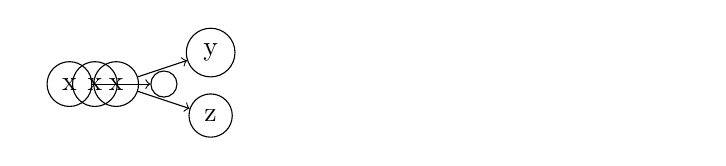
\begin{tikzpicture}
                \graphbox{$L$}{0mm}{0mm}{30mm}{20mm}{0}{0}{
                    \node[draw,circle]  (x) at (-6mm,-12mm) {x};
                    \node[draw,circle] (y) at (6mm,-12mm) {};
                    % \node[draw,circle]  (z) at (6mm,0mm) {};
                    \draw[->]  (x) to (y);
                    % \draw[->] (y) to[bend right=20] (z);
                    % \draw[->]  (z) to[bend right=20] (y);
                }
                \graphbox{$K$}{40mm}{0mm}{30mm}{20mm}{0}{0}{
                    \node[draw,circle]  (x) at (-6mm,-12mm) {x};
                    % \node[draw,circle]  (y) at (6mm,-12mm) {y};
                }
                \graphbox{$R$}{80mm}{0mm}{30mm}{20mm}{0}{0}{
                    \node[draw,circle]  (x) at (-6mm,-12mm) {x};
                        \node[draw,circle]  (y) at (6mm,-8mm) {y};
                        \node[draw,circle]  (z) at (6mm,-16mm) {z};
                        \draw[->]  (x) to (y);
                        \draw[->]  (x) to (z);
                }
                \node () at (35mm,-12mm) {$\leftarrowtail$};
                \node () at (75mm,-12mm) {$\rightarrowtail$};
            \end{tikzpicture}
        }
    \end{center}
    The set \( D(R,X) \) contains exactly two elements $R'$:
    \raisebox{2pt}{ 
        \scalebox{0.6}{\tikz[baseline=-0.5ex]{
        \node [draw,circle] (x) at (0,0) {x};
        \node[draw,circle] (y) at (1,0) {y};
        \draw[->] (x) -- (y) {};
    }}} and $R''$:\raisebox{2pt}{ 
        \scalebox{0.6}{\tikz[baseline=-0.5ex]{
        \node [draw,circle] (x) at (0,0) {x};
        \node[draw,circle] (y) at (1,0) {z};
        \draw[->] (x) -- (y) {};
    }}}. 
    Despite unique monomorphisms \( h_{R'L}: R' \rightarrowtail L \) and \( h_{R''L}: R'' \rightarrowtail L \) preserving interface elements, they fail the third condition of \autoref{def:creates_more_x_on_the_left}. 
    For any rewriting step using this rule, implicitly created $X$-occurrences with the same subgraph of the context have the same corresponding $X$-occurrence. 
\end{example}
 
\begin{example}
    \label{ex:cond4_necessaire}
    Let $X$ be the graph 
    \tikz[baseline=-0.5ex]{ 
            \node (x) at (0,0) {$\bullet$}; 
            \node (y) at (1,0) {$\bullet$};
            \node (z) at (2,0) {$\bullet$};
            \draw[->] (x) -- (y)   {};
    }, which has an isolated node. The following rewriting rule is potentially $X$-increasing.
    \begin{center}
        \resizebox{0.6\textwidth}{!}{
            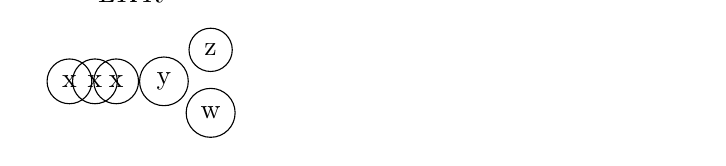
\begin{tikzpicture}
                \graphbox{$L$}{0mm}{0mm}{30mm}{20mm}{0}{0}{
                    \node[draw,circle]  (x) at (-6mm,-10mm) {x};
                    \node[draw,circle] (y) at (6mm,-10mm) {y};
                }
                \graphbox{$K$}{40mm}{0mm}{30mm}{20mm}{0}{0}{
                    \node[draw,circle]  (x) at (-6mm,-10mm) {x};
                }
                \graphbox{$R$}{80mm}{0mm}{30mm}{20mm}{0}{0}{
                    \node[draw,circle]  (x) at (-6mm,-10mm) {x};
                        \node[draw,circle]  (y) at (6mm,-6mm) {z};
                        \node[draw,circle]  (z) at (6mm,-14mm) {w};
                }
                \node () at (35mm,-10mm) {$\leftarrowtail$};
                \node () at (75mm,-10mm) {$\rightarrowtail$};
            \end{tikzpicture}
        }
    \end{center}
    The set \( D(R,X) \) contains exactly two elements $R'$:
    \raisebox{2pt}{\scalebox{0.6}{\tikz[baseline=-0.5ex]{
        \node [draw,circle] (x) at (0,0) {x};
        \node[draw,circle] (y) at (1,0) {z};
        % \draw[->] (x) -- (y) {};
    }}} and $R''$:\raisebox{2pt}{\scalebox{0.6}{\tikz[baseline=-0.5ex]{
        \node [draw,circle] (x) at (0,0) {x};
        \node[draw,circle] (y) at (1,0) {w};
        % \draw[->] (x) -- (y) {};
    }}}. 
    There are unique monomorphisms $h_{R'L}:R' \rightarrowtail L$ and $h_{R''L}:R'' \rightarrowtail L$ preserving interface elements, but they fail the fourth condition of \autoref{def:creates_more_x_on_the_left}.
    For any rewriting step using this rule, implicitly created $X$-occurrences with the same subgraph of the context have the same corresponding $X$-occurrence.
\end{example}
% \subsection{Solution to the key challenge}
% \label{sec:solution_to_the_key_challenge}
% The following lemma ensures that if $\rho$ is $X$-non-increasing, then, for any rewriting step using $\rho$, the cardinality of the set of \( X \)-occurrences implicitly destroyed by the rewriting step is at least as large as the cardinality of the set of \( X \)-occurrences implicitly created by the rewriting step. 
% \subsection{Termination}
% \label{sec:subgraph_counting_antipattern:termination}

We define the following sets of monomorphisms to facilitate the discussion of the termination criterion. They are almost identical to those defined in Notation~\ref{subgraph_counting:notation:mono_sets}. 
\begin{notation}
    \label{antipattern:notation:mono_sets}
  Let \( \mathcal{X}\) be a ruler-graph with underlying graph $X$. The disjoint union of two sets \( S \) and \( S' \) is denoted by \( S \uplus S' \). Let \( X, A, B, G \) be graphs, and let \( \alpha \mathop{\colon} A \mathop{\to} G \) and \( \beta \mathop{\colon} B \mathop{\to} G \) be morphisms as illustrated below:
  \begin{center}
        % \resizebox{0.4\textwidth}{!}{
            \begin{tikzpicture}
            \node (X) at (-1.5,-1) {$X$};
            \node (B) at (2,0) {$A$}; 
            \node (C) at (0,2) {$B$}; 
            \node (D) at (0,0) {$G$}; 
            \draw [>->] (B) to node [above,label,pos=0.45] {$\alpha$} (D); 
            \draw [>->] (C) to node [right,label,pos=0.45] {$\beta$} (D);
            \draw [>->,dashed] (X) to node [above,label,pos=0.45] {$\iota$} (D);
            \draw [>->,dashed] (X) to node [below,label,pos=0.45] {$\zeta$} (B);
            \draw [>->,dashed] (X) to node [above,label,pos=0.45] {$\eta$} (C);
        \end{tikzpicture}
        % }
    \end{center}
     We define the following sets of monomorphisms from $X$ into $G$ based on their interaction with $\alpha$ and $\beta$:    
    \begin{align*}
        \operatorname{Mono}(\mathcal{X},G) &= \operatorname{Mono}(X,G), 
        \\
        \operatorname{Mono}(\mathcal{X},G,\alpha) &= \left\{ \iota \mathop{\colon} X \rightarrowtail G 
        \;\middle|\; 
        \exists \zeta \mathop{\colon} X \rightarrowtail A.\, \iota \mathop{=} \zeta \mathop{\star} \alpha \right\}, 
        \\
        \operatorname{Mono}(\mathcal{X},G,\mathop{\lnot} \alpha) &= \left\{ \iota \mathop{\colon} X \rightarrowtail G 
        \;\middle|\; 
        \nexists \zeta \mathop{\colon} X \rightarrowtail A.\, \iota \mathop{=} \zeta \mathop{\star} \alpha \right\}, 
        \\
        \operatorname{Mono}(\mathcal{X},G,\mathop{\lnot} \alpha, \beta) &= \left\{ 
            \iota \mathop{\colon} X \rightarrowtail G \;\middle|\; 
                \begin{aligned}  
                    &(\nexists \zeta \mathop{\colon} X \rightarrowtail A.\, \iota \mathop{=} \zeta \mathop{\star} \alpha) \\ 
                    &\land (\exists \eta \mathop{\colon} X \rightarrowtail B.\, \iota \mathop{=} \eta \mathop{\star} \beta)
                \end{aligned}
        \right\},
        \\
        \operatorname{Mono}(\mathcal{X},G,\mathop{\lnot} \alpha, \mathop{\lnot} \beta) &= \left\{ 
            \iota \mathop{\colon} X \rightarrowtail G \;\middle|\; 
                \begin{aligned}
                    &(\nexists \zeta \mathop{\colon} X \rightarrowtail A.\, \iota \mathop{=} \zeta \mathop{\star} \alpha) \\
                    &\land (\nexists \eta \mathop{\colon} X \rightarrowtail B.\, \iota \mathop{=} \eta \mathop{\star} \beta)
                \end{aligned}
        \right\}.
    \end{align*}
    For a set $\operatorname{Mono}(\mathcal{X},\dots)$, we write $\operatorname{Mono}(\mathcal{X},\dots)_{\operatorname{NF}}$ for the subset of \( X \)-occurrences whose images are not included in any occurrence of the forbidden context if it exists, and  $\operatorname{Mono}(\mathcal{X},\dots)_{\operatorname{F}}$ for the subset of \( X \)-occurrences whose images are included in some occurrences of the forbidden context if it exists. 
\end{notation}
    Let $\mathcal{X}=(X,\mathcal{C})$ be a ruler-graph and \( \rho \mathop{=} (L \overset{l}{\leftarrowtail} K \overset{r}{\rightarrowtail} R) \) be a rule. 
    Consider the following DPO diagram:
    \begin{center}
        % \resizebox{0.5\textwidth}{!}{
        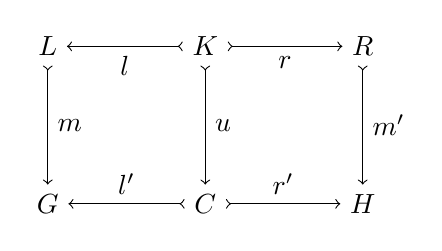
\begin{tikzpicture}
            % [node distance=15mm]
            \node (I) at (0,0) {$K$};
            \node (L)  at (-2,0) {$L$};
            \node (R)  at (2,0) {$R$};
            \node (G)  at (-2,-2) {$G$};
            \node (C)  at (0,-2) {$C$};
            \node (H)  at (2,-2) {$H$};
            \draw [>->] (I) to  node [midway,below] {$l$} (L);
            \draw [>->] (I) to  node [midway,below] {$r$} (R);
            \draw [>->] (L) to node [midway,right] {$m$} (G);
            \draw [>->] (I) to  node [midway,right] {$u$} (C);
            \draw [>->] (R) to  node [midway,right] {$m'$} (H);
            \draw [>->] (C) to node [midway,above] {$l'$} (G);
            \draw [>->] (C) to node [midway,above] {$r'$} (H);
            % \node [at=($(I)!.5!(G)$)] {\normalfont PO};
            % \node [at=($(I)!.5!(H)$)] {\normalfont PO};
        \end{tikzpicture}
        % }
    \end{center}

The set $\operatorname{Mono}(\mathcal{X},G)_{\operatorname{NF}}$ 
decomposes into a union of three disjoint subsets:
\begin{itemize}
    \item $\operatorname{Mono}(\mathcal{X},G,m)_{\operatorname{NF}}$,
    \item $\operatorname{Mono}(\mathcal{X},G,\mathop{\lnot} m, l')_{\operatorname{NF}}$,
    \item $\operatorname{Mono}(\mathcal{X},G,\mathop{\lnot} m, \mathop{\lnot} l')_{\operatorname{NF}}$.
\end{itemize}
% $$
%     \operatorname{Mono}(\mathcal{X},G,m)_{\operatorname{NF}}
%     \uplus
%     \operatorname{Mono}(\mathcal{X},G,\mathop{\lnot} m, l')_{\operatorname{NF}} 
%     \uplus
%     \operatorname{Mono}(\mathcal{X},G,\mathop{\lnot} m, \mathop{\lnot} l')_{\operatorname{NF}}.
% $$
Similarly, the set
 $\operatorname{Mono}(\mathcal{X},H)_{\operatorname{NF}}$ decomposes into a union of three disjoint subsets:
 \begin{itemize}
    \item $\operatorname{Mono}(\mathcal{X},H,m')_{\operatorname{NF}}$,
    \item $\operatorname{Mono}(\mathcal{X},H,\mathop{\lnot} m', r')_{\operatorname{NF}}$,
    \item $\operatorname{Mono}(\mathcal{X},H,\mathop{\lnot} m', \mathop{\lnot} r')_{\operatorname{NF}}$.
 \end{itemize}
\noindent
Thus, the following equality holds:
\begin{flalign}
    &\card{\operatorname{Mono}(\mathcal{X},G)_{\operatorname{NF}}} \mathop{-} 
    \card{\operatorname{Mono}(\mathcal{X},H)_{\operatorname{NF}}} \nonumber
    \\=
    &(\card{\operatorname{Mono}(\mathcal{X},G,m)_{\operatorname{NF}}} 
        \mathop{-}  
    \card{\operatorname{Mono}(\mathcal{X},H,m')_{\operatorname{NF}}}) 
   \mathop{+} \nonumber
    \\
    &(
        \card{\operatorname{Mono}(\mathcal{X},G,\mathop{\lnot} m, l')_{\operatorname{NF}}}
             \mathop{-} 
        \card{\operatorname{Mono}(\mathcal{X},H,\mathop{\lnot} m', r')_{\operatorname{NF}}})\mathop{+} \nonumber \\ 
    &(
        \card{\operatorname{Mono}(\mathcal{X},G,\mathop{\lnot} m, \mathop{\lnot} l')_{\operatorname{NF}}} 
            \mathop{-} 
        \card{\operatorname{Mono}(\mathcal{X},H,\mathop{\lnot} m', \mathop{\lnot} r')_{\operatorname{NF}}} 
    ).\nonumber
\end{flalign}
In the remainder of this section, we suppose that $\rho^{-1}$ is $F$-non-increasing if $\mathcal{C} \mathop{=} \set{f:X \mathop{\rightarrowtail} F}$ and that $\rho$ and $\rho^{-1}$ are $X$-non-increasing.  
The following lemmas provide a lower bound on $\card{\operatorname{Mono}(\mathcal{X},G)_{\operatorname{NF}}} \mathop{-} 
    \card{\operatorname{Mono}(\mathcal{X},H)_{\operatorname{NF}}}$.
% The following lemmas can be used to approximate $\card{\operatorname{Mono}(\mathcal{X},G)_{\operatorname{NF}}} \mathop{-} 
%     \card{\operatorname{Mono}(\mathcal{X},H)_{\operatorname{NF}}}$
\begin{lemma}
    \label{antipattern:lem:xglnotmlp_xhlnotmrp}
        Let \( \rho \mathop{=} (L \overset{l}{\leftarrowtail} K \overset{r}{\rightarrowtail} R) \) be a rule and $\mathcal{X}=(X,\mathcal{C})$ be a ruler-graph. 
        Suppose that $\rho^{-1}$ is $F$-non-increasing if $\mathcal{C} \mathop{=} \set{f:X \rightarrowtail F}$.
        The following inequality holds:
    $$\card{\operatorname{Mono}(\mathcal{X},G,\mathop{\lnot} m, l')_{\operatorname{NF}}} \geq
        \card{\operatorname{Mono}(\mathcal{X},H,\mathop{\lnot} m', r')_{\operatorname{NF}}}.$$
\end{lemma} 
\begin{lemma}
    \label{antipattern:lem:xglnotmlnotlp_xhlnotmrnotrp}
        Let \( \rho \mathop{=} (L \overset{l}{\leftarrowtail} K \overset{r}{\rightarrowtail} R) \) be a rule, and let $\mathcal{X}=(X,\mathcal{C})$ be a ruler-graph. Suppose that $\rho$ and $\rho^{-1}$ are $X$-non-increasing. We have
    $$ 
        \card{\operatorname{Mono}(\mathcal{X},G,\mathop{\lnot} m, \mathop{\lnot} l')_{\operatorname{NF}}} \geq
        \card{\operatorname{Mono}(\mathcal{X},H,\mathop{\lnot} m', \mathop{\lnot} r')_{\operatorname{NF}}}.
    $$
\end{lemma}
Under the assumptions of the above two lemmas, we obtain the following inequality:
 \begin{flalign*}
     \card{\operatorname{Mono}(\mathcal{X},G)_{\operatorname{NF}}} \mathop{-} 
     \card{\operatorname{Mono}(\mathcal{X},H)_{\operatorname{NF}}} 
     \geq
     \card{\operatorname{Mono}(\mathcal{X},G,m)_{\operatorname{NF}}} \mathop{-} \card{\operatorname{Mono}(\mathcal{X},H,m')_{\operatorname{NF}}}.
 \end{flalign*}

 The following introduce a subset of $\operatorname{Mono}(\mathcal{X},L)_{\operatorname{NF}}$ that consists of $X$-occurrences whose images are not included in any occurrence of the forbidden context in $L$,
    but, in some rewriting step $G \mathop{\Rightarrow}_\rho^m H$, their images may possibly be included in some occurrence of the forbidden context in the host graph $G$.
\begin{definition}
    \label{antipattern:def:gamma_l_rho_x}
    Let $\mathcal{X}=(X,\mathcal{C})$ be a ruler-graph, and let \( \rho \mathop{=} (L \overset{l}{\leftarrowtail} K \overset{r}{\rightarrowtail} R) \) be a rule.
    Define $\Gamma(\operatorname{Mono}(\mathcal{X},L)_{\operatorname{NF}})\subseteq \operatorname{Mono}(\mathcal{X},L)_{\operatorname{NF}}$ as follows:
    $\Gamma(\operatorname{Mono}(\mathcal{X},L)_{\operatorname{NF}}) \mathop{=} \emptyset$ if $\mathcal{C} \mathop{=} \emptyset$, and if $\mathcal{C} \mathop{=} \set{f\mathop{\colon}X \rightarrowtail F}$, then a monomorphism $h_{XL} \mathop{\colon} X \rightarrowtail L$ is in $\Gamma(\operatorname{Mono}(\mathcal{X},L)_{\operatorname{NF}})$ if and only if the following hold:
    \begin{itemize}
        \item there does not exist $h_{FL}:F \rightarrowtail L$ such that $f \mathop{\star} h_{FL} \mathop{=} h_{XL}$, and
         \item  
         there are a graph $C$, a monomorphism $K \overset{u}{\rightarrowtail} C$, and the pushout $L \overset{m}{\rightarrowtail} G \overset{l'}{\leftarrowtail} C$ of $L \overset{l}{\leftarrowtail} K \overset{u}{\rightarrowtail} C$ such that
         there is a monomorphism $h_{FG} \mathop{\colon} F \rightarrowtail G$ satisfying
         $h_{XL} \mathop{\star} m \mathop{=} h_{XF} \mathop{\star} h_{FG}$. 
      \begin{center}
        % \resizebox{0.4\textwidth}{!}{
            \begin{tikzpicture}
                    \node (k) at (0,1) {K};
                    \node (l) at (-2,1) {L};
                    \node (c) at (0,-1) {C};
                    \node (g) at (-2,-1) {G};
                    \node (x) at (-4,-2) {X};
                    \node (f) at (-2,-2) {F};
                    \draw[<-<]  (l) -- (k) node [midway,below] {$l$};
                    \draw[>->] (c) -- (g) node [midway, above] {$l'$};
                    \draw[>->] (l) -- (g) node[midway, right] {$m$};
                    \draw[>->] (k) -- (c) node[midway, left] {$u$};
                    \draw[>->] (x) -- (l) node[midway, left] {$h_{XL}$};
                    \draw[>->] (x) -- (f) node[midway, above] {$f$};
                    \draw[>->] (f) -- (g) node[midway, right] {$h_{FG}$};
                    \node () [at=($(l)!0.5!(c)$)] {$PO$};
                \end{tikzpicture}
        %  }
        \end{center}
    \end{itemize}
%    \trackedtext{Intuitively, $\Lambda(\mathcal{X},\rho)$ is the number of $X$-occurrences in $L$ ...}
\end{definition}
We define $\Lambda(\mathcal{X},\rho) \overset{\operatorname{def}}{=} (\card{\operatorname{Mono}(\mathcal{X},L)_{\operatorname{NF}}} \mathop{-} 
    \card{\Gamma(\operatorname{Mono}(\mathcal{X},L)_{\operatorname{NF}})}) -
   \card{\operatorname{Mono}(\mathcal{X},R)_{\operatorname{NF}}}$ to improve the readability of the subsequent discussion.

Note that in the category \textbf{Graph}, the pushout of two arrows always exists~\cite[p.188]{corradini1997algebraic}. This justifies the existence of the pushout square in the second condition of the above definition.
Furthermore, since $X$ and the forbidden context (if exists) are finite graphs, $\Lambda(\mathcal{X},\rho)$ can be precisely computed. Consequently, it provides a lower bound for the change in the number of $X$-occurrences in a rewriting step using $\rho$, as shown in the following lemma whose proof is given in~\textsection~\ref{antipattern:proof:lem:xgm_xhmp_xl_xr}.

% \begin{lemma}
%     \label{lem:decomp_w_u}
%     \ \newline
%     \noindent
%     \begin{minipage}{0.7\textwidth}
%         Let $X$ be a ruler-graph. For a pushout square as shown on the right, we have 
%         % $\card{\operatorname{Mono}(X, B)} \mathop{=} \card{\operatorname{Mono}(X, D, \beta')}$ and $\card{\operatorname{Mono}(X, C, \mathop{\lnot} \beta)} \mathop{=} \card{\operatorname{Mono}(X, D, \mathop{\lnot} \beta', \alpha')}$.
%         \begin{flalign*}
%             \card{\operatorname{Mono}(X, B)} &= \card{\operatorname{Mono}(X, D, \beta')}
%             \\
%             \card{\operatorname{Mono}(X, C, \mathop{\lnot} \beta)} &= \card{\operatorname{Mono}(X, D, \mathop{\lnot} \beta', \alpha')}
%         \end{flalign*}
%     \end{minipage}
%     \hfill
%     \begin{minipage}{0.3\textwidth}
%         \hfill
%         \begin{tikzpicture}
%             \node (A) {$A$};
%             \node [below of=A] (B) {$B$}; 
%             \node [left of=A] (C) {$C$}; 
%             \node [left of=B] (D) {$D$}; 
%             \begin{scope}[nodes=rectangle]          
%             \draw [>->] (A) to node [right,label,pos=0.5] {$\alpha$} (B);
%             \draw [>->] (A) to node [above,label,pos=0.5] {$\beta$} (C);
%             \draw [>->] (B) to node [below,label,pos=0.45] {$\beta'$} (D); 
%             \draw [>->] (C) to node [left,label,pos=0.45] {$\alpha'$} (D);
%             \end{scope}
%         \end{tikzpicture}
%     \end{minipage} 
% \end{lemma}
% \begin{proof}
%     See the Appendix,~\autoref{proof:dcomp_w_u}.
%  \end{proof}
% \begin{lemma}
%     \label{lem:xgm_xhmp_xl_xr}
%     % If the number of $X$-occurrences that are not  included in any occurrences of forbidden context $F \mathop{\in} F_x$ in a $\rho$-rewriting step is predictable, then
%     $
%         \card{\operatorname{Mono}(\mathcal{X},G,m)_{\operatorname{NF}}} \mathop{-} 
%         \card{\operatorname{Mono}(\mathcal{X},H,m')_{\operatorname{NF}}} 
%         \mathop{\geq} 
%         \card{\operatorname{Mono}(X,L)} -
%         \card{\operatorname{Mono}(X,R)}
%     $
% \end{lemma}
% \begin{proof}
%     See the Appendix, \textsection~\ref{proof:lem:xgm_xhmp_xl_xr}.
%  \end{proof}

\begin{lemma}
    \label{antipattern:lem:xgm_xhmp_xl_xr}
     Let $\mathcal{X}$ be a ruler-graph, and let \( \rho \mathop{=} (L \overset{l}{\leftarrowtail} K \overset{r}{\rightarrowtail} R) \) be a rule. 
   We have
    \begin{flalign*}
        &\card{\operatorname{Mono}(\mathcal{X},G,m)_{\operatorname{NF}}} \mathop{-} 
        \card{\operatorname{Mono}(\mathcal{X},H,m')_{\operatorname{NF}}} 
        \geq
        \Lambda(\mathcal{X},\rho).
    \end{flalign*}
\end{lemma}
 Thus, by the unnumbered equation preceding Definition~\ref{antipattern:def:gamma_l_rho_x}, the following inequality holds:
 \begin{flalign}
         \card{\operatorname{Mono}(\mathcal{X},G)_{\operatorname{NF}}} \mathop{-} 
     \card{\operatorname{Mono}(\mathcal{X},H)_{\operatorname{NF}}} 
     \mathop{\geq} 
    \Lambda(\mathcal{X},\rho).
     \label{eq:mono_x_g_nf_mono_x_h_nf_geq}
 \end{flalign}
Consequently, we have  
\begin{flalign*}
    w_{s_\mathbb{X}}(G) \mathop{-} w_{s_\mathbb{X}}(H)
   \overset{\operatorname{def}}{=}&\sum_{\mathcal{X} \mathop{\in} \mathbb{X}}^{}s_\mathbb{X}(\mathcal{X}) \mathop{*} m_X(G) \mathop{-} \sum_{\mathcal{X} \mathop{\in} \mathbb{X}}^{}s_\mathbb{X}(\mathcal{X}) \mathop{*} m_X(H)
   \\
   \overset{\operatorname{def}}{=}&\sum_{\mathcal{X} \mathop{\in} \mathbb{X}}^{}s_\mathbb{X}(\mathcal{X}) \mathop{*} |\operatorname{Mono}(\mathcal{X},G)_{\operatorname{NF}}| \mathop{-} \sum_{\mathcal{X} \mathop{\in} \mathbb{X}}^{}s_\mathbb{X}(\mathcal{X}) \mathop{*} |\operatorname{Mono}(\mathcal{X},H)_{\operatorname{NF}}|
   \\
   =&\sum_{\mathcal{X} \mathop{\in} \mathbb{X}}^{}s_\mathbb{X}(\mathcal{X}) \mathop{*} \left( \card{\operatorname{Mono}(\mathcal{X},G)_{\operatorname{NF}}} \mathop{-} 
   \card{\operatorname{Mono}(\mathcal{X},H)_{\operatorname{NF}}} \right)
   \\
   \geq&\sum_{\mathcal{X} \mathop{\in} \mathbb{X}}^{}s_\mathbb{X}(\mathcal{X}) \mathop{*} \Lambda(\mathcal{X},\rho).
   \hspace{2cm} \text{by~\eqref{eq:mono_x_g_nf_mono_x_h_nf_geq}}
\end{flalign*} 
This proves the following key lemma of this section.
\begin{lemma}[Decreasing step]
    \label{antipattern:lem:w_g_geq_w_h_leq}
    Let $\rho \mathop{=} (L \overset{l}{\leftarrowtail} K \overset{r}{\rightarrowtail} R)$ be an injective DPO rewriting rule,
    \( \mathbb{X} \) a set of ruler-graphs,
    \( s_{\mathbb{X}} \mathop{\colon} \mathbb{X} \mathop{\to} \mathbb{N} \) a weight function,
    and \( G \mathop{\Rightarrow}_{\rho,\mathfrak{M}} H \) a rewriting step. 
    Suppose that for every \( \mathcal{X}=(X,\mathcal{C}) \mathop{\in} \mathbb{X} \), 
    % the number of $X$-occurrences that are not included in any occurrences of forbidden context $F \mathop{\in} F_x$ in a $\rho$-rewriting step is predictable,
    $\rho$ is $X$-non-increasing, and if $\mathcal{C}= \set{f:X \rightarrowtail F}$ then $\rho^{-1}$ is $X$-non-increasing and $F$-non-increasing. The following inequality holds:
     $$
        w_{s_\mathbb{X}}(G) \mathop{-} w_{s_\mathbb{X}}(H) 
        \mathop{\geq} 
        \sum_{\mathcal{X} \mathop{\in} \mathbb{X}}^{}s_\mathbb{X}(\mathcal{X}) \mathop{*} \Lambda(\mathcal{X},\rho).
    $$
\end{lemma}
Finally, our main result follows.
\begin{theorem}[Termination] 
    \label{antipattern:thm:termination_grs} 
    Let \(\mathcal{A}\) and \(\mathcal{B}\) be sets of injective DPO rewriting rules, $\mathbb{X}$ a set of ruler-graphs, and $s_\mathbb{X}$ a weight function. If the following conditions hold:
    \begin{enumerate}
        \item  for every $\rho \mathop{\in} \mathcal{A} \mathop{\cup} \mathcal{B}$ and for every \( \mathcal{X} = (X, \mathcal{C}) \mathop{\in} \mathbb{X} \), 
        % the number of $X$-occurrences that are not included in any occurrences of the forbidden context $F \mathop{\in} F_x$ in a $\rho$-rewriting step is predictable,
        $\rho$ is $X$-non-increasing, and if $\mathcal{C}= \set{f:X \rightarrowtail F}$ then $\rho^{-1}$ is $X$-non-increasing and $F$-non-increasing, and
        % $\rho^{-1}$ is $F$-non-increasing if $\mathcal{X}= (X,f:X \rightarrowtail F)$ and, $\rho$ and $\rho^{-1}$ are $X$-non-increasing
        \item for every \(\rho \mathop{\in} \mathcal{A}\), we have
        % \( w_{s_\mathbb{X}}(lhs(\rho)) \mathop{>} w_{s_\mathbb{X}}(rhs(\rho)) \),
        $ \sum_{\mathcal{X} \mathop{\in} \mathbb{X}}^{}s_\mathbb{X}(\mathcal{X}) \mathop{*} 
            \Lambda(\mathcal{X},\rho) \mathop{>} 0 $, and
        \item for every \(\rho \mathop{\in} \mathcal{B}\), we have   
        % \( w_{s_\mathbb{X}}(lhs(\rho)) \mathop{\geq} w_{s_\mathbb{X}}(rhs(\rho)) \).
        $ 
            \sum_{\mathcal{X} \mathop{\in} \mathbb{X}}^{}s_\mathbb{X}(\mathcal{X}) \mathop{*} \Lambda(\mathcal{X},\rho) \mathop{\geq} 0 
        $,
    \end{enumerate}
    then \(\mathop{\Rightarrow}_{\mathcal{A},\mathcal{M}}\) terminates relative to \(\mathop{\Rightarrow}_{\mathcal{B},\mathcal{M}}\).
\end{theorem}
\begin{remark}
    This work focuses on deriving sufficient conditions for termination, deferring the construction of ruler-graphs to future work.
\end{remark} 
 